% Created by tikzDevice version 0.10.1 on 2016-09-06 19:52:25
% !TEX encoding = UTF-8 Unicode
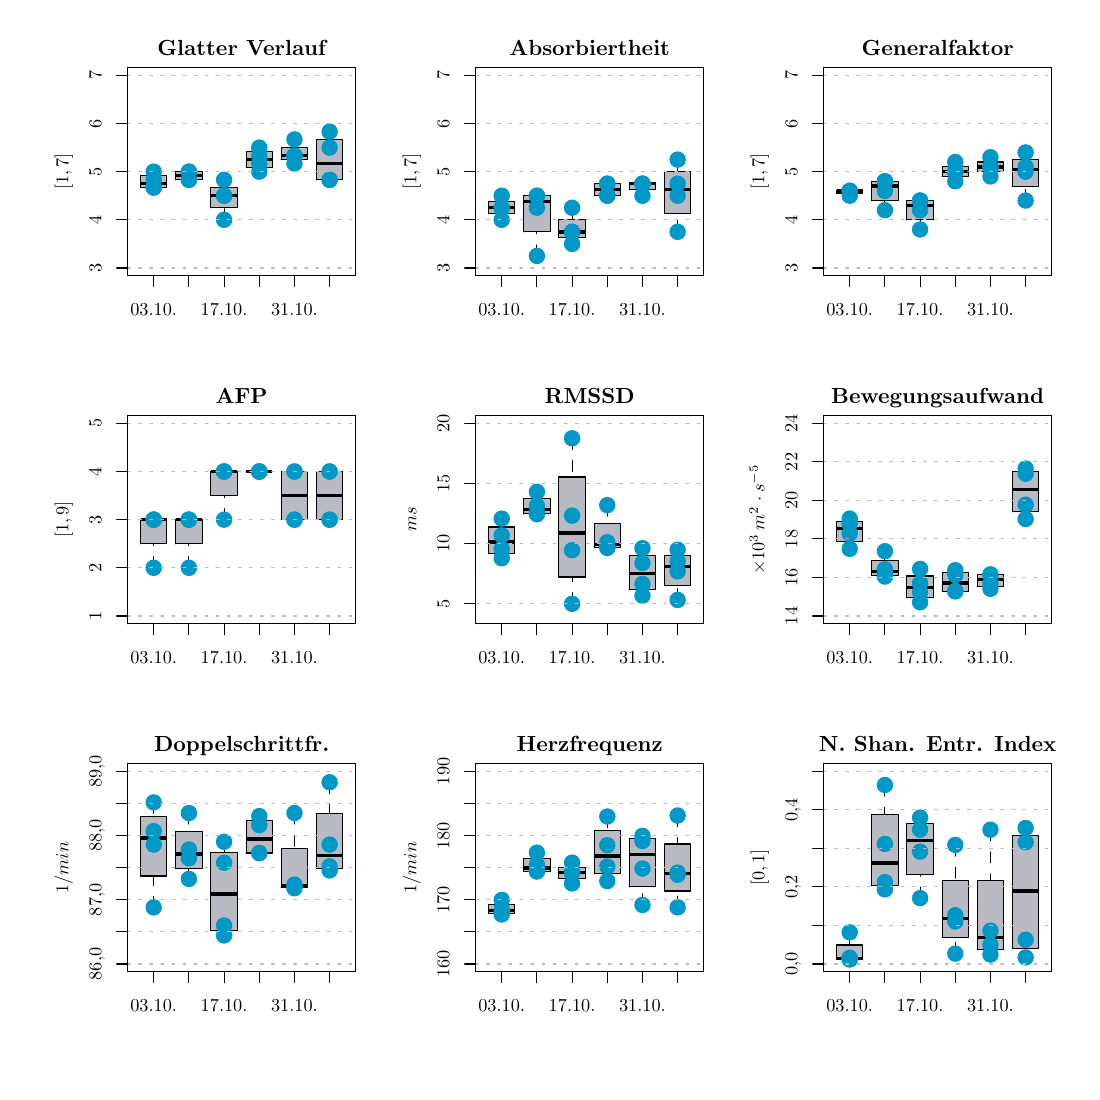
\begin{tikzpicture}[x=1pt,y=1pt]
\definecolor{fillColor}{RGB}{255,255,255}
\path[use as bounding box,fill=fillColor] (0,0) rectangle (377.25,377.25);
\begin{scope}
\path[clip] ( 36.13,287.63) rectangle (118.52,362.80);
\definecolor{fillColor}{RGB}{186,187,194}

\path[fill=fillColor] ( 40.78,319.47) --
	( 50.31,319.47) --
	( 50.31,323.74) --
	( 40.78,323.74) --
	cycle;
\definecolor{drawColor}{RGB}{0,0,0}

\path[draw=drawColor,line width= 1.2pt,line join=round] ( 40.78,320.87) -- ( 50.31,320.87);

\path[draw=drawColor,line width= 0.4pt,dash pattern=on 4pt off 4pt ,line join=round,line cap=round] ( 45.54,319.47) -- ( 45.54,319.47);

\path[draw=drawColor,line width= 0.4pt,dash pattern=on 4pt off 4pt ,line join=round,line cap=round] ( 45.54,325.21) -- ( 45.54,323.74);

\path[draw=drawColor,line width= 0.4pt,line join=round,line cap=round] ( 43.16,319.47) -- ( 47.93,319.47);

\path[draw=drawColor,line width= 0.4pt,line join=round,line cap=round] ( 43.16,325.21) -- ( 47.93,325.21);

\path[draw=drawColor,line width= 0.4pt,line join=round,line cap=round] ( 40.78,319.47) --
	( 50.31,319.47) --
	( 50.31,323.74) --
	( 40.78,323.74) --
	( 40.78,319.47);

\path[fill=fillColor] ( 53.49,322.26) --
	( 63.03,322.26) --
	( 63.03,325.21) --
	( 53.49,325.21) --
	cycle;

\path[draw=drawColor,line width= 1.2pt,line join=round] ( 53.49,323.74) -- ( 63.03,323.74);

\path[draw=drawColor,line width= 0.4pt,dash pattern=on 4pt off 4pt ,line join=round,line cap=round] ( 58.26,322.26) -- ( 58.26,322.26);

\path[draw=drawColor,line width= 0.4pt,dash pattern=on 4pt off 4pt ,line join=round,line cap=round] ( 58.26,325.21) -- ( 58.26,325.21);

\path[draw=drawColor,line width= 0.4pt,line join=round,line cap=round] ( 55.87,322.26) -- ( 60.64,322.26);

\path[draw=drawColor,line width= 0.4pt,line join=round,line cap=round] ( 55.87,325.21) -- ( 60.64,325.21);

\path[draw=drawColor,line width= 0.4pt,line join=round,line cap=round] ( 53.49,322.26) --
	( 63.03,322.26) --
	( 63.03,325.21) --
	( 53.49,325.21) --
	( 53.49,322.26);

\path[fill=fillColor] ( 66.20,312.17) --
	( 75.74,312.17) --
	( 75.74,319.39) --
	( 66.20,319.39) --
	cycle;

\path[draw=drawColor,line width= 1.2pt,line join=round] ( 66.20,316.52) -- ( 75.74,316.52);

\path[draw=drawColor,line width= 0.4pt,dash pattern=on 4pt off 4pt ,line join=round,line cap=round] ( 70.97,307.82) -- ( 70.97,312.17);

\path[draw=drawColor,line width= 0.4pt,dash pattern=on 4pt off 4pt ,line join=round,line cap=round] ( 70.97,322.26) -- ( 70.97,319.39);

\path[draw=drawColor,line width= 0.4pt,line join=round,line cap=round] ( 68.59,307.82) -- ( 73.36,307.82);

\path[draw=drawColor,line width= 0.4pt,line join=round,line cap=round] ( 68.59,322.26) -- ( 73.36,322.26);

\path[draw=drawColor,line width= 0.4pt,line join=round,line cap=round] ( 66.20,312.17) --
	( 75.74,312.17) --
	( 75.74,319.39) --
	( 66.20,319.39) --
	( 66.20,312.17);

\path[fill=fillColor] ( 78.92,326.69) --
	( 88.45,326.69) --
	( 88.45,332.44) --
	( 78.92,332.44) --
	cycle;

\path[draw=drawColor,line width= 1.2pt,line join=round] ( 78.92,329.56) -- ( 88.45,329.56);

\path[draw=drawColor,line width= 0.4pt,dash pattern=on 4pt off 4pt ,line join=round,line cap=round] ( 83.69,325.21) -- ( 83.69,326.69);

\path[draw=drawColor,line width= 0.4pt,dash pattern=on 4pt off 4pt ,line join=round,line cap=round] ( 83.69,333.91) -- ( 83.69,332.44);

\path[draw=drawColor,line width= 0.4pt,line join=round,line cap=round] ( 81.30,325.21) -- ( 86.07,325.21);

\path[draw=drawColor,line width= 0.4pt,line join=round,line cap=round] ( 81.30,333.91) -- ( 86.07,333.91);

\path[draw=drawColor,line width= 0.4pt,line join=round,line cap=round] ( 78.92,326.69) --
	( 88.45,326.69) --
	( 88.45,332.44) --
	( 78.92,332.44) --
	( 78.92,326.69);

\path[fill=fillColor] ( 91.63,329.56) --
	(101.17,329.56) --
	(101.17,333.91) --
	( 91.63,333.91) --
	cycle;

\path[draw=drawColor,line width= 1.2pt,line join=round] ( 91.63,330.96) -- (101.17,330.96);

\path[draw=drawColor,line width= 0.4pt,dash pattern=on 4pt off 4pt ,line join=round,line cap=round] ( 96.40,328.17) -- ( 96.40,329.56);

\path[draw=drawColor,line width= 0.4pt,dash pattern=on 4pt off 4pt ,line join=round,line cap=round] ( 96.40,336.87) -- ( 96.40,333.91);

\path[draw=drawColor,line width= 0.4pt,line join=round,line cap=round] ( 94.02,328.17) -- ( 98.78,328.17);

\path[draw=drawColor,line width= 0.4pt,line join=round,line cap=round] ( 94.02,336.87) -- ( 98.78,336.87);

\path[draw=drawColor,line width= 0.4pt,line join=round,line cap=round] ( 91.63,329.56) --
	(101.17,329.56) --
	(101.17,333.91) --
	( 91.63,333.91) --
	( 91.63,329.56);

\path[fill=fillColor] (104.35,322.26) --
	(113.88,322.26) --
	(113.88,336.78) --
	(104.35,336.78) --
	cycle;

\path[draw=drawColor,line width= 1.2pt,line join=round] (104.35,328.09) -- (113.88,328.09);

\path[draw=drawColor,line width= 0.4pt,dash pattern=on 4pt off 4pt ,line join=round,line cap=round] (109.11,322.26) -- (109.11,322.26);

\path[draw=drawColor,line width= 0.4pt,dash pattern=on 4pt off 4pt ,line join=round,line cap=round] (109.11,339.66) -- (109.11,336.78);

\path[draw=drawColor,line width= 0.4pt,line join=round,line cap=round] (106.73,322.26) -- (111.50,322.26);

\path[draw=drawColor,line width= 0.4pt,line join=round,line cap=round] (106.73,339.66) -- (111.50,339.66);

\path[draw=drawColor,line width= 0.4pt,line join=round,line cap=round] (104.35,322.26) --
	(113.88,322.26) --
	(113.88,336.78) --
	(104.35,336.78) --
	(104.35,322.26);
\end{scope}
\begin{scope}
\path[clip] (  0.00,  0.00) rectangle (377.25,377.25);
\definecolor{drawColor}{RGB}{0,0,0}

\path[draw=drawColor,line width= 0.4pt,line join=round,line cap=round] ( 45.54,287.63) -- (109.11,287.63);

\path[draw=drawColor,line width= 0.4pt,line join=round,line cap=round] ( 45.54,287.63) -- ( 45.54,283.67);

\path[draw=drawColor,line width= 0.4pt,line join=round,line cap=round] ( 58.26,287.63) -- ( 58.26,283.67);

\path[draw=drawColor,line width= 0.4pt,line join=round,line cap=round] ( 70.97,287.63) -- ( 70.97,283.67);

\path[draw=drawColor,line width= 0.4pt,line join=round,line cap=round] ( 83.69,287.63) -- ( 83.69,283.67);

\path[draw=drawColor,line width= 0.4pt,line join=round,line cap=round] ( 96.40,287.63) -- ( 96.40,283.67);

\path[draw=drawColor,line width= 0.4pt,line join=round,line cap=round] (109.11,287.63) -- (109.11,283.67);

\node[text=drawColor,anchor=base,inner sep=0pt, outer sep=0pt, scale=  0.66] at ( 45.54,273.38) {03.10.};

\node[text=drawColor,anchor=base,inner sep=0pt, outer sep=0pt, scale=  0.66] at ( 70.97,273.38) {17.10.};

\node[text=drawColor,anchor=base,inner sep=0pt, outer sep=0pt, scale=  0.66] at ( 96.40,273.38) {31.10.};

\path[draw=drawColor,line width= 0.4pt,line join=round,line cap=round] ( 36.13,290.42) -- ( 36.13,360.01);

\path[draw=drawColor,line width= 0.4pt,line join=round,line cap=round] ( 36.13,290.42) -- ( 32.17,290.42);

\path[draw=drawColor,line width= 0.4pt,line join=round,line cap=round] ( 36.13,307.82) -- ( 32.17,307.82);

\path[draw=drawColor,line width= 0.4pt,line join=round,line cap=round] ( 36.13,325.21) -- ( 32.17,325.21);

\path[draw=drawColor,line width= 0.4pt,line join=round,line cap=round] ( 36.13,342.61) -- ( 32.17,342.61);

\path[draw=drawColor,line width= 0.4pt,line join=round,line cap=round] ( 36.13,360.01) -- ( 32.17,360.01);

\node[text=drawColor,rotate= 90.00,anchor=base,inner sep=0pt, outer sep=0pt, scale=  0.66] at ( 26.63,290.42) {3};

\node[text=drawColor,rotate= 90.00,anchor=base,inner sep=0pt, outer sep=0pt, scale=  0.66] at ( 26.63,307.82) {4};

\node[text=drawColor,rotate= 90.00,anchor=base,inner sep=0pt, outer sep=0pt, scale=  0.66] at ( 26.63,325.21) {5};

\node[text=drawColor,rotate= 90.00,anchor=base,inner sep=0pt, outer sep=0pt, scale=  0.66] at ( 26.63,342.61) {6};

\node[text=drawColor,rotate= 90.00,anchor=base,inner sep=0pt, outer sep=0pt, scale=  0.66] at ( 26.63,360.01) {7};
\end{scope}
\begin{scope}
\path[clip] (  0.00,251.50) rectangle (125.75,377.25);
\definecolor{drawColor}{RGB}{0,0,0}

\node[text=drawColor,anchor=base,inner sep=0pt, outer sep=0pt, scale=  0.79] at ( 77.33,367.29) {\bfseries Glatter Verlauf};

\node[text=drawColor,rotate= 90.00,anchor=base,inner sep=0pt, outer sep=0pt, scale=  0.66] at ( 14.75,325.21) {$[1, 7]$};
\end{scope}
\begin{scope}
\path[clip] (  0.00,  0.00) rectangle (377.25,377.25);
\definecolor{drawColor}{RGB}{0,0,0}

\path[draw=drawColor,line width= 0.4pt,line join=round,line cap=round] ( 36.13,287.63) --
	(118.52,287.63) --
	(118.52,362.80) --
	( 36.13,362.80) --
	( 36.13,287.63);
\end{scope}
\begin{scope}
\path[clip] ( 36.13,287.63) rectangle (118.52,362.80);
\definecolor{fillColor}{RGB}{0,152,199}

\path[fill=fillColor] ( 45.54,325.21) circle (  2.97);

\path[fill=fillColor] ( 45.54,322.26) circle (  2.97);

\path[fill=fillColor] ( 45.54,319.47) circle (  2.97);

\path[fill=fillColor] ( 45.54,319.47) circle (  2.97);

\path[fill=fillColor] ( 58.26,322.26) circle (  2.97);

\path[fill=fillColor] ( 58.26,325.21) circle (  2.97);

\path[fill=fillColor] ( 58.26,325.21) circle (  2.97);

\path[fill=fillColor] ( 58.26,322.26) circle (  2.97);

\path[fill=fillColor] ( 70.97,322.26) circle (  2.97);

\path[fill=fillColor] ( 70.97,316.52) circle (  2.97);

\path[fill=fillColor] ( 70.97,307.82) circle (  2.97);

\path[fill=fillColor] ( 70.97,316.52) circle (  2.97);

\path[fill=fillColor] ( 83.69,330.96) circle (  2.97);

\path[fill=fillColor] ( 83.69,325.21) circle (  2.97);

\path[fill=fillColor] ( 83.69,333.91) circle (  2.97);

\path[fill=fillColor] ( 83.69,328.17) circle (  2.97);

\path[fill=fillColor] ( 96.40,330.96) circle (  2.97);

\path[fill=fillColor] ( 96.40,328.17) circle (  2.97);

\path[fill=fillColor] ( 96.40,330.96) circle (  2.97);

\path[fill=fillColor] ( 96.40,336.87) circle (  2.97);

\path[fill=fillColor] (109.11,339.66) circle (  2.97);

\path[fill=fillColor] (109.11,333.91) circle (  2.97);

\path[fill=fillColor] (109.11,322.26) circle (  2.97);

\path[fill=fillColor] (109.11,322.26) circle (  2.97);
\definecolor{drawColor}{RGB}{186,187,194}

\path[draw=drawColor,line width= 0.4pt,dash pattern=on 1pt off 3pt ,line join=round,line cap=round] ( 36.13,290.42) -- (118.52,290.42);

\path[draw=drawColor,line width= 0.4pt,dash pattern=on 1pt off 3pt ,line join=round,line cap=round] ( 36.13,307.82) -- (118.52,307.82);

\path[draw=drawColor,line width= 0.4pt,dash pattern=on 1pt off 3pt ,line join=round,line cap=round] ( 36.13,325.21) -- (118.52,325.21);

\path[draw=drawColor,line width= 0.4pt,dash pattern=on 1pt off 3pt ,line join=round,line cap=round] ( 36.13,342.61) -- (118.52,342.61);

\path[draw=drawColor,line width= 0.4pt,dash pattern=on 1pt off 3pt ,line join=round,line cap=round] ( 36.13,360.01) -- (118.52,360.01);
\end{scope}
\begin{scope}
\path[clip] (  0.00,  0.00) rectangle (377.25,377.25);
\definecolor{drawColor}{RGB}{0,0,0}

\path[draw=drawColor,line width= 0.4pt,line join=round,line cap=round] ( 36.13,287.63) --
	(118.52,287.63) --
	(118.52,362.80) --
	( 36.13,362.80) --
	( 36.13,287.63);
\end{scope}
\begin{scope}
\path[clip] (161.88,287.63) rectangle (244.27,362.80);
\definecolor{fillColor}{RGB}{186,187,194}

\path[fill=fillColor] (166.53,309.99) --
	(176.06,309.99) --
	(176.06,314.34) --
	(166.53,314.34) --
	cycle;
\definecolor{drawColor}{RGB}{0,0,0}

\path[draw=drawColor,line width= 1.2pt,line join=round] (166.53,312.17) -- (176.06,312.17);

\path[draw=drawColor,line width= 0.4pt,dash pattern=on 4pt off 4pt ,line join=round,line cap=round] (171.29,307.82) -- (171.29,309.99);

\path[draw=drawColor,line width= 0.4pt,dash pattern=on 4pt off 4pt ,line join=round,line cap=round] (171.29,316.52) -- (171.29,314.34);

\path[draw=drawColor,line width= 0.4pt,line join=round,line cap=round] (168.91,307.82) -- (173.68,307.82);

\path[draw=drawColor,line width= 0.4pt,line join=round,line cap=round] (168.91,316.52) -- (173.68,316.52);

\path[draw=drawColor,line width= 0.4pt,line join=round,line cap=round] (166.53,309.99) --
	(176.06,309.99) --
	(176.06,314.34) --
	(166.53,314.34) --
	(166.53,309.99);

\path[fill=fillColor] (179.24,303.47) --
	(188.78,303.47) --
	(188.78,316.52) --
	(179.24,316.52) --
	cycle;

\path[draw=drawColor,line width= 1.2pt,line join=round] (179.24,314.34) -- (188.78,314.34);

\path[draw=drawColor,line width= 0.4pt,dash pattern=on 4pt off 4pt ,line join=round,line cap=round] (184.01,294.77) -- (184.01,303.47);

\path[draw=drawColor,line width= 0.4pt,dash pattern=on 4pt off 4pt ,line join=round,line cap=round] (184.01,316.52) -- (184.01,316.52);

\path[draw=drawColor,line width= 0.4pt,line join=round,line cap=round] (181.62,294.77) -- (186.39,294.77);

\path[draw=drawColor,line width= 0.4pt,line join=round,line cap=round] (181.62,316.52) -- (186.39,316.52);

\path[draw=drawColor,line width= 0.4pt,line join=round,line cap=round] (179.24,303.47) --
	(188.78,303.47) --
	(188.78,316.52) --
	(179.24,316.52) --
	(179.24,303.47);

\path[fill=fillColor] (191.95,301.29) --
	(201.49,301.29) --
	(201.49,307.82) --
	(191.95,307.82) --
	cycle;

\path[draw=drawColor,line width= 1.2pt,line join=round] (191.95,303.47) -- (201.49,303.47);

\path[draw=drawColor,line width= 0.4pt,dash pattern=on 4pt off 4pt ,line join=round,line cap=round] (196.72,299.12) -- (196.72,301.29);

\path[draw=drawColor,line width= 0.4pt,dash pattern=on 4pt off 4pt ,line join=round,line cap=round] (196.72,312.17) -- (196.72,307.82);

\path[draw=drawColor,line width= 0.4pt,line join=round,line cap=round] (194.34,299.12) -- (199.11,299.12);

\path[draw=drawColor,line width= 0.4pt,line join=round,line cap=round] (194.34,312.17) -- (199.11,312.17);

\path[draw=drawColor,line width= 0.4pt,line join=round,line cap=round] (191.95,301.29) --
	(201.49,301.29) --
	(201.49,307.82) --
	(191.95,307.82) --
	(191.95,301.29);

\path[fill=fillColor] (204.67,316.52) --
	(214.20,316.52) --
	(214.20,320.87) --
	(204.67,320.87) --
	cycle;

\path[draw=drawColor,line width= 1.2pt,line join=round] (204.67,318.69) -- (214.20,318.69);

\path[draw=drawColor,line width= 0.4pt,dash pattern=on 4pt off 4pt ,line join=round,line cap=round] (209.44,316.52) -- (209.44,316.52);

\path[draw=drawColor,line width= 0.4pt,dash pattern=on 4pt off 4pt ,line join=round,line cap=round] (209.44,320.87) -- (209.44,320.87);

\path[draw=drawColor,line width= 0.4pt,line join=round,line cap=round] (207.05,316.52) -- (211.82,316.52);

\path[draw=drawColor,line width= 0.4pt,line join=round,line cap=round] (207.05,320.87) -- (211.82,320.87);

\path[draw=drawColor,line width= 0.4pt,line join=round,line cap=round] (204.67,316.52) --
	(214.20,316.52) --
	(214.20,320.87) --
	(204.67,320.87) --
	(204.67,316.52);

\path[fill=fillColor] (217.38,318.69) --
	(226.92,318.69) --
	(226.92,320.87) --
	(217.38,320.87) --
	cycle;

\path[draw=drawColor,line width= 1.2pt,line join=round] (217.38,320.87) -- (226.92,320.87);

\path[draw=drawColor,line width= 0.4pt,dash pattern=on 4pt off 4pt ,line join=round,line cap=round] (222.15,316.52) -- (222.15,318.69);

\path[draw=drawColor,line width= 0.4pt,dash pattern=on 4pt off 4pt ,line join=round,line cap=round] (222.15,320.87) -- (222.15,320.87);

\path[draw=drawColor,line width= 0.4pt,line join=round,line cap=round] (219.77,316.52) -- (224.53,316.52);

\path[draw=drawColor,line width= 0.4pt,line join=round,line cap=round] (219.77,320.87) -- (224.53,320.87);

\path[draw=drawColor,line width= 0.4pt,line join=round,line cap=round] (217.38,318.69) --
	(226.92,318.69) --
	(226.92,320.87) --
	(217.38,320.87) --
	(217.38,318.69);

\path[fill=fillColor] (230.10,309.99) --
	(239.63,309.99) --
	(239.63,325.21) --
	(230.10,325.21) --
	cycle;

\path[draw=drawColor,line width= 1.2pt,line join=round] (230.10,318.69) -- (239.63,318.69);

\path[draw=drawColor,line width= 0.4pt,dash pattern=on 4pt off 4pt ,line join=round,line cap=round] (234.86,303.47) -- (234.86,309.99);

\path[draw=drawColor,line width= 0.4pt,dash pattern=on 4pt off 4pt ,line join=round,line cap=round] (234.86,329.56) -- (234.86,325.21);

\path[draw=drawColor,line width= 0.4pt,line join=round,line cap=round] (232.48,303.47) -- (237.25,303.47);

\path[draw=drawColor,line width= 0.4pt,line join=round,line cap=round] (232.48,329.56) -- (237.25,329.56);

\path[draw=drawColor,line width= 0.4pt,line join=round,line cap=round] (230.10,309.99) --
	(239.63,309.99) --
	(239.63,325.21) --
	(230.10,325.21) --
	(230.10,309.99);
\end{scope}
\begin{scope}
\path[clip] (  0.00,  0.00) rectangle (377.25,377.25);
\definecolor{drawColor}{RGB}{0,0,0}

\path[draw=drawColor,line width= 0.4pt,line join=round,line cap=round] (171.29,287.63) -- (234.86,287.63);

\path[draw=drawColor,line width= 0.4pt,line join=round,line cap=round] (171.29,287.63) -- (171.29,283.67);

\path[draw=drawColor,line width= 0.4pt,line join=round,line cap=round] (184.01,287.63) -- (184.01,283.67);

\path[draw=drawColor,line width= 0.4pt,line join=round,line cap=round] (196.72,287.63) -- (196.72,283.67);

\path[draw=drawColor,line width= 0.4pt,line join=round,line cap=round] (209.44,287.63) -- (209.44,283.67);

\path[draw=drawColor,line width= 0.4pt,line join=round,line cap=round] (222.15,287.63) -- (222.15,283.67);

\path[draw=drawColor,line width= 0.4pt,line join=round,line cap=round] (234.86,287.63) -- (234.86,283.67);

\node[text=drawColor,anchor=base,inner sep=0pt, outer sep=0pt, scale=  0.66] at (171.29,273.38) {03.10.};

\node[text=drawColor,anchor=base,inner sep=0pt, outer sep=0pt, scale=  0.66] at (196.72,273.38) {17.10.};

\node[text=drawColor,anchor=base,inner sep=0pt, outer sep=0pt, scale=  0.66] at (222.15,273.38) {31.10.};

\path[draw=drawColor,line width= 0.4pt,line join=round,line cap=round] (161.88,290.42) -- (161.88,360.01);

\path[draw=drawColor,line width= 0.4pt,line join=round,line cap=round] (161.88,290.42) -- (157.92,290.42);

\path[draw=drawColor,line width= 0.4pt,line join=round,line cap=round] (161.88,307.82) -- (157.92,307.82);

\path[draw=drawColor,line width= 0.4pt,line join=round,line cap=round] (161.88,325.21) -- (157.92,325.21);

\path[draw=drawColor,line width= 0.4pt,line join=round,line cap=round] (161.88,342.61) -- (157.92,342.61);

\path[draw=drawColor,line width= 0.4pt,line join=round,line cap=round] (161.88,360.01) -- (157.92,360.01);

\node[text=drawColor,rotate= 90.00,anchor=base,inner sep=0pt, outer sep=0pt, scale=  0.66] at (152.38,290.42) {3};

\node[text=drawColor,rotate= 90.00,anchor=base,inner sep=0pt, outer sep=0pt, scale=  0.66] at (152.38,307.82) {4};

\node[text=drawColor,rotate= 90.00,anchor=base,inner sep=0pt, outer sep=0pt, scale=  0.66] at (152.38,325.21) {5};

\node[text=drawColor,rotate= 90.00,anchor=base,inner sep=0pt, outer sep=0pt, scale=  0.66] at (152.38,342.61) {6};

\node[text=drawColor,rotate= 90.00,anchor=base,inner sep=0pt, outer sep=0pt, scale=  0.66] at (152.38,360.01) {7};
\end{scope}
\begin{scope}
\path[clip] (125.75,251.50) rectangle (251.50,377.25);
\definecolor{drawColor}{RGB}{0,0,0}

\node[text=drawColor,anchor=base,inner sep=0pt, outer sep=0pt, scale=  0.79] at (203.08,367.29) {\bfseries Absorbiertheit};

\node[text=drawColor,rotate= 90.00,anchor=base,inner sep=0pt, outer sep=0pt, scale=  0.66] at (140.50,325.21) {$[1, 7]$};
\end{scope}
\begin{scope}
\path[clip] (  0.00,  0.00) rectangle (377.25,377.25);
\definecolor{drawColor}{RGB}{0,0,0}

\path[draw=drawColor,line width= 0.4pt,line join=round,line cap=round] (161.88,287.63) --
	(244.27,287.63) --
	(244.27,362.80) --
	(161.88,362.80) --
	(161.88,287.63);
\end{scope}
\begin{scope}
\path[clip] (161.88,287.63) rectangle (244.27,362.80);
\definecolor{fillColor}{RGB}{0,152,199}

\path[fill=fillColor] (171.29,307.82) circle (  2.97);

\path[fill=fillColor] (171.29,312.17) circle (  2.97);

\path[fill=fillColor] (171.29,316.52) circle (  2.97);

\path[fill=fillColor] (171.29,312.17) circle (  2.97);

\path[fill=fillColor] (184.01,294.77) circle (  2.97);

\path[fill=fillColor] (184.01,316.52) circle (  2.97);

\path[fill=fillColor] (184.01,316.52) circle (  2.97);

\path[fill=fillColor] (184.01,312.17) circle (  2.97);

\path[fill=fillColor] (196.72,303.47) circle (  2.97);

\path[fill=fillColor] (196.72,303.47) circle (  2.97);

\path[fill=fillColor] (196.72,299.12) circle (  2.97);

\path[fill=fillColor] (196.72,312.17) circle (  2.97);

\path[fill=fillColor] (209.44,316.52) circle (  2.97);

\path[fill=fillColor] (209.44,316.52) circle (  2.97);

\path[fill=fillColor] (209.44,320.87) circle (  2.97);

\path[fill=fillColor] (209.44,320.87) circle (  2.97);

\path[fill=fillColor] (222.15,320.87) circle (  2.97);

\path[fill=fillColor] (222.15,316.52) circle (  2.97);

\path[fill=fillColor] (222.15,320.87) circle (  2.97);

\path[fill=fillColor] (222.15,320.87) circle (  2.97);

\path[fill=fillColor] (234.86,320.87) circle (  2.97);

\path[fill=fillColor] (234.86,316.52) circle (  2.97);

\path[fill=fillColor] (234.86,329.56) circle (  2.97);

\path[fill=fillColor] (234.86,303.47) circle (  2.97);
\definecolor{drawColor}{RGB}{186,187,194}

\path[draw=drawColor,line width= 0.4pt,dash pattern=on 1pt off 3pt ,line join=round,line cap=round] (161.88,290.42) -- (244.27,290.42);

\path[draw=drawColor,line width= 0.4pt,dash pattern=on 1pt off 3pt ,line join=round,line cap=round] (161.88,307.82) -- (244.27,307.82);

\path[draw=drawColor,line width= 0.4pt,dash pattern=on 1pt off 3pt ,line join=round,line cap=round] (161.88,325.21) -- (244.27,325.21);

\path[draw=drawColor,line width= 0.4pt,dash pattern=on 1pt off 3pt ,line join=round,line cap=round] (161.88,342.61) -- (244.27,342.61);

\path[draw=drawColor,line width= 0.4pt,dash pattern=on 1pt off 3pt ,line join=round,line cap=round] (161.88,360.01) -- (244.27,360.01);
\end{scope}
\begin{scope}
\path[clip] (  0.00,  0.00) rectangle (377.25,377.25);
\definecolor{drawColor}{RGB}{0,0,0}

\path[draw=drawColor,line width= 0.4pt,line join=round,line cap=round] (161.88,287.63) --
	(244.27,287.63) --
	(244.27,362.80) --
	(161.88,362.80) --
	(161.88,287.63);
\end{scope}
\begin{scope}
\path[clip] (287.63,287.63) rectangle (370.02,362.80);
\definecolor{fillColor}{RGB}{186,187,194}

\path[fill=fillColor] (292.28,317.39) --
	(301.81,317.39) --
	(301.81,318.26) --
	(292.28,318.26) --
	cycle;
\definecolor{drawColor}{RGB}{0,0,0}

\path[draw=drawColor,line width= 1.2pt,line join=round] (292.28,318.26) -- (301.81,318.26);

\path[draw=drawColor,line width= 0.4pt,dash pattern=on 4pt off 4pt ,line join=round,line cap=round] (297.04,316.52) -- (297.04,317.39);

\path[draw=drawColor,line width= 0.4pt,dash pattern=on 4pt off 4pt ,line join=round,line cap=round] (297.04,318.26) -- (297.04,318.26);

\path[draw=drawColor,line width= 0.4pt,line join=round,line cap=round] (294.66,316.52) -- (299.43,316.52);

\path[draw=drawColor,line width= 0.4pt,line join=round,line cap=round] (294.66,318.26) -- (299.43,318.26);

\path[draw=drawColor,line width= 0.4pt,line join=round,line cap=round] (292.28,317.39) --
	(301.81,317.39) --
	(301.81,318.26) --
	(292.28,318.26) --
	(292.28,317.39);

\path[fill=fillColor] (304.99,314.78) --
	(314.53,314.78) --
	(314.53,321.74) --
	(304.99,321.74) --
	cycle;

\path[draw=drawColor,line width= 1.2pt,line join=round] (304.99,320.00) -- (314.53,320.00);

\path[draw=drawColor,line width= 0.4pt,dash pattern=on 4pt off 4pt ,line join=round,line cap=round] (309.76,311.30) -- (309.76,314.78);

\path[draw=drawColor,line width= 0.4pt,dash pattern=on 4pt off 4pt ,line join=round,line cap=round] (309.76,321.74) -- (309.76,321.74);

\path[draw=drawColor,line width= 0.4pt,line join=round,line cap=round] (307.37,311.30) -- (312.14,311.30);

\path[draw=drawColor,line width= 0.4pt,line join=round,line cap=round] (307.37,321.74) -- (312.14,321.74);

\path[draw=drawColor,line width= 0.4pt,line join=round,line cap=round] (304.99,314.78) --
	(314.53,314.78) --
	(314.53,321.74) --
	(304.99,321.74) --
	(304.99,314.78);

\path[fill=fillColor] (317.70,307.82) --
	(327.24,307.82) --
	(327.24,314.78) --
	(317.70,314.78) --
	cycle;

\path[draw=drawColor,line width= 1.2pt,line join=round] (317.70,313.04) -- (327.24,313.04);

\path[draw=drawColor,line width= 0.4pt,dash pattern=on 4pt off 4pt ,line join=round,line cap=round] (322.47,304.34) -- (322.47,307.82);

\path[draw=drawColor,line width= 0.4pt,dash pattern=on 4pt off 4pt ,line join=round,line cap=round] (322.47,314.78) -- (322.47,314.78);

\path[draw=drawColor,line width= 0.4pt,line join=round,line cap=round] (320.09,304.34) -- (324.86,304.34);

\path[draw=drawColor,line width= 0.4pt,line join=round,line cap=round] (320.09,314.78) -- (324.86,314.78);

\path[draw=drawColor,line width= 0.4pt,line join=round,line cap=round] (317.70,307.82) --
	(327.24,307.82) --
	(327.24,314.78) --
	(317.70,314.78) --
	(317.70,307.82);

\path[fill=fillColor] (330.42,323.48) --
	(339.95,323.48) --
	(339.95,326.95) --
	(330.42,326.95) --
	cycle;

\path[draw=drawColor,line width= 1.2pt,line join=round] (330.42,325.21) -- (339.95,325.21);

\path[draw=drawColor,line width= 0.4pt,dash pattern=on 4pt off 4pt ,line join=round,line cap=round] (335.19,321.74) -- (335.19,323.48);

\path[draw=drawColor,line width= 0.4pt,dash pattern=on 4pt off 4pt ,line join=round,line cap=round] (335.19,328.69) -- (335.19,326.95);

\path[draw=drawColor,line width= 0.4pt,line join=round,line cap=round] (332.80,321.74) -- (337.57,321.74);

\path[draw=drawColor,line width= 0.4pt,line join=round,line cap=round] (332.80,328.69) -- (337.57,328.69);

\path[draw=drawColor,line width= 0.4pt,line join=round,line cap=round] (330.42,323.48) --
	(339.95,323.48) --
	(339.95,326.95) --
	(330.42,326.95) --
	(330.42,323.48);

\path[fill=fillColor] (343.13,325.21) --
	(352.67,325.21) --
	(352.67,328.69) --
	(343.13,328.69) --
	cycle;

\path[draw=drawColor,line width= 1.2pt,line join=round] (343.13,326.95) -- (352.67,326.95);

\path[draw=drawColor,line width= 0.4pt,dash pattern=on 4pt off 4pt ,line join=round,line cap=round] (347.90,323.48) -- (347.90,325.21);

\path[draw=drawColor,line width= 0.4pt,dash pattern=on 4pt off 4pt ,line join=round,line cap=round] (347.90,330.43) -- (347.90,328.69);

\path[draw=drawColor,line width= 0.4pt,line join=round,line cap=round] (345.52,323.48) -- (350.28,323.48);

\path[draw=drawColor,line width= 0.4pt,line join=round,line cap=round] (345.52,330.43) -- (350.28,330.43);

\path[draw=drawColor,line width= 0.4pt,line join=round,line cap=round] (343.13,325.21) --
	(352.67,325.21) --
	(352.67,328.69) --
	(343.13,328.69) --
	(343.13,325.21);

\path[fill=fillColor] (355.85,320.00) --
	(365.38,320.00) --
	(365.38,329.56) --
	(355.85,329.56) --
	cycle;

\path[draw=drawColor,line width= 1.2pt,line join=round] (355.85,326.08) -- (365.38,326.08);

\path[draw=drawColor,line width= 0.4pt,dash pattern=on 4pt off 4pt ,line join=round,line cap=round] (360.61,314.78) -- (360.61,320.00);

\path[draw=drawColor,line width= 0.4pt,dash pattern=on 4pt off 4pt ,line join=round,line cap=round] (360.61,332.17) -- (360.61,329.56);

\path[draw=drawColor,line width= 0.4pt,line join=round,line cap=round] (358.23,314.78) -- (363.00,314.78);

\path[draw=drawColor,line width= 0.4pt,line join=round,line cap=round] (358.23,332.17) -- (363.00,332.17);

\path[draw=drawColor,line width= 0.4pt,line join=round,line cap=round] (355.85,320.00) --
	(365.38,320.00) --
	(365.38,329.56) --
	(355.85,329.56) --
	(355.85,320.00);
\end{scope}
\begin{scope}
\path[clip] (  0.00,  0.00) rectangle (377.25,377.25);
\definecolor{drawColor}{RGB}{0,0,0}

\path[draw=drawColor,line width= 0.4pt,line join=round,line cap=round] (297.04,287.63) -- (360.61,287.63);

\path[draw=drawColor,line width= 0.4pt,line join=round,line cap=round] (297.04,287.63) -- (297.04,283.67);

\path[draw=drawColor,line width= 0.4pt,line join=round,line cap=round] (309.76,287.63) -- (309.76,283.67);

\path[draw=drawColor,line width= 0.4pt,line join=round,line cap=round] (322.47,287.63) -- (322.47,283.67);

\path[draw=drawColor,line width= 0.4pt,line join=round,line cap=round] (335.19,287.63) -- (335.19,283.67);

\path[draw=drawColor,line width= 0.4pt,line join=round,line cap=round] (347.90,287.63) -- (347.90,283.67);

\path[draw=drawColor,line width= 0.4pt,line join=round,line cap=round] (360.61,287.63) -- (360.61,283.67);

\node[text=drawColor,anchor=base,inner sep=0pt, outer sep=0pt, scale=  0.66] at (297.04,273.38) {03.10.};

\node[text=drawColor,anchor=base,inner sep=0pt, outer sep=0pt, scale=  0.66] at (322.47,273.38) {17.10.};

\node[text=drawColor,anchor=base,inner sep=0pt, outer sep=0pt, scale=  0.66] at (347.90,273.38) {31.10.};

\path[draw=drawColor,line width= 0.4pt,line join=round,line cap=round] (287.63,290.42) -- (287.63,360.01);

\path[draw=drawColor,line width= 0.4pt,line join=round,line cap=round] (287.63,290.42) -- (283.67,290.42);

\path[draw=drawColor,line width= 0.4pt,line join=round,line cap=round] (287.63,307.82) -- (283.67,307.82);

\path[draw=drawColor,line width= 0.4pt,line join=round,line cap=round] (287.63,325.21) -- (283.67,325.21);

\path[draw=drawColor,line width= 0.4pt,line join=round,line cap=round] (287.63,342.61) -- (283.67,342.61);

\path[draw=drawColor,line width= 0.4pt,line join=round,line cap=round] (287.63,360.01) -- (283.67,360.01);

\node[text=drawColor,rotate= 90.00,anchor=base,inner sep=0pt, outer sep=0pt, scale=  0.66] at (278.13,290.42) {3};

\node[text=drawColor,rotate= 90.00,anchor=base,inner sep=0pt, outer sep=0pt, scale=  0.66] at (278.13,307.82) {4};

\node[text=drawColor,rotate= 90.00,anchor=base,inner sep=0pt, outer sep=0pt, scale=  0.66] at (278.13,325.21) {5};

\node[text=drawColor,rotate= 90.00,anchor=base,inner sep=0pt, outer sep=0pt, scale=  0.66] at (278.13,342.61) {6};

\node[text=drawColor,rotate= 90.00,anchor=base,inner sep=0pt, outer sep=0pt, scale=  0.66] at (278.13,360.01) {7};
\end{scope}
\begin{scope}
\path[clip] (251.50,251.50) rectangle (377.25,377.25);
\definecolor{drawColor}{RGB}{0,0,0}

\node[text=drawColor,anchor=base,inner sep=0pt, outer sep=0pt, scale=  0.79] at (328.83,367.29) {\bfseries Generalfaktor};

\node[text=drawColor,rotate= 90.00,anchor=base,inner sep=0pt, outer sep=0pt, scale=  0.66] at (266.25,325.21) {$[1, 7]$};
\end{scope}
\begin{scope}
\path[clip] (  0.00,  0.00) rectangle (377.25,377.25);
\definecolor{drawColor}{RGB}{0,0,0}

\path[draw=drawColor,line width= 0.4pt,line join=round,line cap=round] (287.63,287.63) --
	(370.02,287.63) --
	(370.02,362.80) --
	(287.63,362.80) --
	(287.63,287.63);
\end{scope}
\begin{scope}
\path[clip] (287.63,287.63) rectangle (370.02,362.80);
\definecolor{fillColor}{RGB}{0,152,199}

\path[fill=fillColor] (297.04,318.26) circle (  2.97);

\path[fill=fillColor] (297.04,318.26) circle (  2.97);

\path[fill=fillColor] (297.04,318.26) circle (  2.97);

\path[fill=fillColor] (297.04,316.52) circle (  2.97);

\path[fill=fillColor] (309.76,311.30) circle (  2.97);

\path[fill=fillColor] (309.76,321.74) circle (  2.97);

\path[fill=fillColor] (309.76,321.74) circle (  2.97);

\path[fill=fillColor] (309.76,318.26) circle (  2.97);

\path[fill=fillColor] (322.47,314.78) circle (  2.97);

\path[fill=fillColor] (322.47,311.30) circle (  2.97);

\path[fill=fillColor] (322.47,304.34) circle (  2.97);

\path[fill=fillColor] (322.47,314.78) circle (  2.97);

\path[fill=fillColor] (335.19,325.21) circle (  2.97);

\path[fill=fillColor] (335.19,321.74) circle (  2.97);

\path[fill=fillColor] (335.19,328.69) circle (  2.97);

\path[fill=fillColor] (335.19,325.21) circle (  2.97);

\path[fill=fillColor] (347.90,326.95) circle (  2.97);

\path[fill=fillColor] (347.90,323.48) circle (  2.97);

\path[fill=fillColor] (347.90,326.95) circle (  2.97);

\path[fill=fillColor] (347.90,330.43) circle (  2.97);

\path[fill=fillColor] (360.61,332.17) circle (  2.97);

\path[fill=fillColor] (360.61,326.95) circle (  2.97);

\path[fill=fillColor] (360.61,325.21) circle (  2.97);

\path[fill=fillColor] (360.61,314.78) circle (  2.97);
\definecolor{drawColor}{RGB}{186,187,194}

\path[draw=drawColor,line width= 0.4pt,dash pattern=on 1pt off 3pt ,line join=round,line cap=round] (287.63,290.42) -- (370.02,290.42);

\path[draw=drawColor,line width= 0.4pt,dash pattern=on 1pt off 3pt ,line join=round,line cap=round] (287.63,307.82) -- (370.02,307.82);

\path[draw=drawColor,line width= 0.4pt,dash pattern=on 1pt off 3pt ,line join=round,line cap=round] (287.63,325.21) -- (370.02,325.21);

\path[draw=drawColor,line width= 0.4pt,dash pattern=on 1pt off 3pt ,line join=round,line cap=round] (287.63,342.61) -- (370.02,342.61);

\path[draw=drawColor,line width= 0.4pt,dash pattern=on 1pt off 3pt ,line join=round,line cap=round] (287.63,360.01) -- (370.02,360.01);
\end{scope}
\begin{scope}
\path[clip] (  0.00,  0.00) rectangle (377.25,377.25);
\definecolor{drawColor}{RGB}{0,0,0}

\path[draw=drawColor,line width= 0.4pt,line join=round,line cap=round] (287.63,287.63) --
	(370.02,287.63) --
	(370.02,362.80) --
	(287.63,362.80) --
	(287.63,287.63);
\end{scope}
\begin{scope}
\path[clip] ( 36.13,161.88) rectangle (118.52,237.05);
\definecolor{fillColor}{RGB}{186,187,194}

\path[fill=fillColor] ( 40.78,190.77) --
	( 50.31,190.77) --
	( 50.31,199.47) --
	( 40.78,199.47) --
	cycle;
\definecolor{drawColor}{RGB}{0,0,0}

\path[draw=drawColor,line width= 1.2pt,line join=round] ( 40.78,199.47) -- ( 50.31,199.47);

\path[draw=drawColor,line width= 0.4pt,dash pattern=on 4pt off 4pt ,line join=round,line cap=round] ( 45.54,182.07) -- ( 45.54,190.77);

\path[draw=drawColor,line width= 0.4pt,dash pattern=on 4pt off 4pt ,line join=round,line cap=round] ( 45.54,199.47) -- ( 45.54,199.47);

\path[draw=drawColor,line width= 0.4pt,line join=round,line cap=round] ( 43.16,182.07) -- ( 47.93,182.07);

\path[draw=drawColor,line width= 0.4pt,line join=round,line cap=round] ( 43.16,199.47) -- ( 47.93,199.47);

\path[draw=drawColor,line width= 0.4pt,line join=round,line cap=round] ( 40.78,190.77) --
	( 50.31,190.77) --
	( 50.31,199.47) --
	( 40.78,199.47) --
	( 40.78,190.77);

\path[fill=fillColor] ( 53.49,190.77) --
	( 63.03,190.77) --
	( 63.03,199.47) --
	( 53.49,199.47) --
	cycle;

\path[draw=drawColor,line width= 1.2pt,line join=round] ( 53.49,199.47) -- ( 63.03,199.47);

\path[draw=drawColor,line width= 0.4pt,dash pattern=on 4pt off 4pt ,line join=round,line cap=round] ( 58.26,182.07) -- ( 58.26,190.77);

\path[draw=drawColor,line width= 0.4pt,dash pattern=on 4pt off 4pt ,line join=round,line cap=round] ( 58.26,199.47) -- ( 58.26,199.47);

\path[draw=drawColor,line width= 0.4pt,line join=round,line cap=round] ( 55.87,182.07) -- ( 60.64,182.07);

\path[draw=drawColor,line width= 0.4pt,line join=round,line cap=round] ( 55.87,199.47) -- ( 60.64,199.47);

\path[draw=drawColor,line width= 0.4pt,line join=round,line cap=round] ( 53.49,190.77) --
	( 63.03,190.77) --
	( 63.03,199.47) --
	( 53.49,199.47) --
	( 53.49,190.77);

\path[fill=fillColor] ( 66.20,208.16) --
	( 75.74,208.16) --
	( 75.74,216.86) --
	( 66.20,216.86) --
	cycle;

\path[draw=drawColor,line width= 1.2pt,line join=round] ( 66.20,216.86) -- ( 75.74,216.86);

\path[draw=drawColor,line width= 0.4pt,dash pattern=on 4pt off 4pt ,line join=round,line cap=round] ( 70.97,199.47) -- ( 70.97,208.16);

\path[draw=drawColor,line width= 0.4pt,dash pattern=on 4pt off 4pt ,line join=round,line cap=round] ( 70.97,216.86) -- ( 70.97,216.86);

\path[draw=drawColor,line width= 0.4pt,line join=round,line cap=round] ( 68.59,199.47) -- ( 73.36,199.47);

\path[draw=drawColor,line width= 0.4pt,line join=round,line cap=round] ( 68.59,216.86) -- ( 73.36,216.86);

\path[draw=drawColor,line width= 0.4pt,line join=round,line cap=round] ( 66.20,208.16) --
	( 75.74,208.16) --
	( 75.74,216.86) --
	( 66.20,216.86) --
	( 66.20,208.16);

\path[fill=fillColor] ( 78.92,216.86) --
	( 88.45,216.86) --
	( 88.45,216.86) --
	( 78.92,216.86) --
	cycle;

\path[draw=drawColor,line width= 1.2pt,line join=round] ( 78.92,216.86) -- ( 88.45,216.86);

\path[draw=drawColor,line width= 0.4pt,dash pattern=on 4pt off 4pt ,line join=round,line cap=round] ( 83.69,216.86) -- ( 83.69,216.86);

\path[draw=drawColor,line width= 0.4pt,dash pattern=on 4pt off 4pt ,line join=round,line cap=round] ( 83.69,216.86) -- ( 83.69,216.86);

\path[draw=drawColor,line width= 0.4pt,line join=round,line cap=round] ( 81.30,216.86) -- ( 86.07,216.86);

\path[draw=drawColor,line width= 0.4pt,line join=round,line cap=round] ( 81.30,216.86) -- ( 86.07,216.86);

\path[draw=drawColor,line width= 0.4pt,line join=round,line cap=round] ( 78.92,216.86) --
	( 88.45,216.86) --
	( 88.45,216.86) --
	( 78.92,216.86) --
	( 78.92,216.86);

\path[fill=fillColor] ( 91.63,199.47) --
	(101.17,199.47) --
	(101.17,216.86) --
	( 91.63,216.86) --
	cycle;

\path[draw=drawColor,line width= 1.2pt,line join=round] ( 91.63,208.16) -- (101.17,208.16);

\path[draw=drawColor,line width= 0.4pt,dash pattern=on 4pt off 4pt ,line join=round,line cap=round] ( 96.40,199.47) -- ( 96.40,199.47);

\path[draw=drawColor,line width= 0.4pt,dash pattern=on 4pt off 4pt ,line join=round,line cap=round] ( 96.40,216.86) -- ( 96.40,216.86);

\path[draw=drawColor,line width= 0.4pt,line join=round,line cap=round] ( 94.02,199.47) -- ( 98.78,199.47);

\path[draw=drawColor,line width= 0.4pt,line join=round,line cap=round] ( 94.02,216.86) -- ( 98.78,216.86);

\path[draw=drawColor,line width= 0.4pt,line join=round,line cap=round] ( 91.63,199.47) --
	(101.17,199.47) --
	(101.17,216.86) --
	( 91.63,216.86) --
	( 91.63,199.47);

\path[fill=fillColor] (104.35,199.47) --
	(113.88,199.47) --
	(113.88,216.86) --
	(104.35,216.86) --
	cycle;

\path[draw=drawColor,line width= 1.2pt,line join=round] (104.35,208.16) -- (113.88,208.16);

\path[draw=drawColor,line width= 0.4pt,dash pattern=on 4pt off 4pt ,line join=round,line cap=round] (109.11,199.47) -- (109.11,199.47);

\path[draw=drawColor,line width= 0.4pt,dash pattern=on 4pt off 4pt ,line join=round,line cap=round] (109.11,216.86) -- (109.11,216.86);

\path[draw=drawColor,line width= 0.4pt,line join=round,line cap=round] (106.73,199.47) -- (111.50,199.47);

\path[draw=drawColor,line width= 0.4pt,line join=round,line cap=round] (106.73,216.86) -- (111.50,216.86);

\path[draw=drawColor,line width= 0.4pt,line join=round,line cap=round] (104.35,199.47) --
	(113.88,199.47) --
	(113.88,216.86) --
	(104.35,216.86) --
	(104.35,199.47);
\end{scope}
\begin{scope}
\path[clip] (  0.00,  0.00) rectangle (377.25,377.25);
\definecolor{drawColor}{RGB}{0,0,0}

\path[draw=drawColor,line width= 0.4pt,line join=round,line cap=round] ( 45.54,161.88) -- (109.11,161.88);

\path[draw=drawColor,line width= 0.4pt,line join=round,line cap=round] ( 45.54,161.88) -- ( 45.54,157.92);

\path[draw=drawColor,line width= 0.4pt,line join=round,line cap=round] ( 58.26,161.88) -- ( 58.26,157.92);

\path[draw=drawColor,line width= 0.4pt,line join=round,line cap=round] ( 70.97,161.88) -- ( 70.97,157.92);

\path[draw=drawColor,line width= 0.4pt,line join=round,line cap=round] ( 83.69,161.88) -- ( 83.69,157.92);

\path[draw=drawColor,line width= 0.4pt,line join=round,line cap=round] ( 96.40,161.88) -- ( 96.40,157.92);

\path[draw=drawColor,line width= 0.4pt,line join=round,line cap=round] (109.11,161.88) -- (109.11,157.92);

\node[text=drawColor,anchor=base,inner sep=0pt, outer sep=0pt, scale=  0.66] at ( 45.54,147.63) {03.10.};

\node[text=drawColor,anchor=base,inner sep=0pt, outer sep=0pt, scale=  0.66] at ( 70.97,147.63) {17.10.};

\node[text=drawColor,anchor=base,inner sep=0pt, outer sep=0pt, scale=  0.66] at ( 96.40,147.63) {31.10.};

\path[draw=drawColor,line width= 0.4pt,line join=round,line cap=round] ( 36.13,164.67) -- ( 36.13,234.26);

\path[draw=drawColor,line width= 0.4pt,line join=round,line cap=round] ( 36.13,164.67) -- ( 32.17,164.67);

\path[draw=drawColor,line width= 0.4pt,line join=round,line cap=round] ( 36.13,182.07) -- ( 32.17,182.07);

\path[draw=drawColor,line width= 0.4pt,line join=round,line cap=round] ( 36.13,199.47) -- ( 32.17,199.47);

\path[draw=drawColor,line width= 0.4pt,line join=round,line cap=round] ( 36.13,216.86) -- ( 32.17,216.86);

\path[draw=drawColor,line width= 0.4pt,line join=round,line cap=round] ( 36.13,234.26) -- ( 32.17,234.26);

\node[text=drawColor,rotate= 90.00,anchor=base,inner sep=0pt, outer sep=0pt, scale=  0.66] at ( 26.63,164.67) {1};

\node[text=drawColor,rotate= 90.00,anchor=base,inner sep=0pt, outer sep=0pt, scale=  0.66] at ( 26.63,182.07) {2};

\node[text=drawColor,rotate= 90.00,anchor=base,inner sep=0pt, outer sep=0pt, scale=  0.66] at ( 26.63,199.47) {3};

\node[text=drawColor,rotate= 90.00,anchor=base,inner sep=0pt, outer sep=0pt, scale=  0.66] at ( 26.63,216.86) {4};

\node[text=drawColor,rotate= 90.00,anchor=base,inner sep=0pt, outer sep=0pt, scale=  0.66] at ( 26.63,234.26) {5};
\end{scope}
\begin{scope}
\path[clip] (  0.00,125.75) rectangle (125.75,251.50);
\definecolor{drawColor}{RGB}{0,0,0}

\node[text=drawColor,anchor=base,inner sep=0pt, outer sep=0pt, scale=  0.79] at ( 77.33,241.54) {\bfseries AFP};

\node[text=drawColor,rotate= 90.00,anchor=base,inner sep=0pt, outer sep=0pt, scale=  0.66] at ( 14.75,199.47) {$[1, 9]$};
\end{scope}
\begin{scope}
\path[clip] (  0.00,  0.00) rectangle (377.25,377.25);
\definecolor{drawColor}{RGB}{0,0,0}

\path[draw=drawColor,line width= 0.4pt,line join=round,line cap=round] ( 36.13,161.88) --
	(118.52,161.88) --
	(118.52,237.05) --
	( 36.13,237.05) --
	( 36.13,161.88);
\end{scope}
\begin{scope}
\path[clip] ( 36.13,161.88) rectangle (118.52,237.05);
\definecolor{fillColor}{RGB}{0,152,199}

\path[fill=fillColor] ( 45.54,182.07) circle (  2.97);

\path[fill=fillColor] ( 45.54,199.47) circle (  2.97);

\path[fill=fillColor] ( 45.54,199.47) circle (  2.97);

\path[fill=fillColor] ( 45.54,199.47) circle (  2.97);

\path[fill=fillColor] ( 58.26,182.07) circle (  2.97);

\path[fill=fillColor] ( 58.26,199.47) circle (  2.97);

\path[fill=fillColor] ( 58.26,199.47) circle (  2.97);

\path[fill=fillColor] ( 58.26,199.47) circle (  2.97);

\path[fill=fillColor] ( 70.97,199.47) circle (  2.97);

\path[fill=fillColor] ( 70.97,216.86) circle (  2.97);

\path[fill=fillColor] ( 70.97,216.86) circle (  2.97);

\path[fill=fillColor] ( 70.97,216.86) circle (  2.97);

\path[fill=fillColor] ( 83.69,216.86) circle (  2.97);

\path[fill=fillColor] ( 83.69,216.86) circle (  2.97);

\path[fill=fillColor] ( 83.69,216.86) circle (  2.97);

\path[fill=fillColor] ( 83.69,216.86) circle (  2.97);

\path[fill=fillColor] ( 96.40,199.47) circle (  2.97);

\path[fill=fillColor] ( 96.40,199.47) circle (  2.97);

\path[fill=fillColor] ( 96.40,216.86) circle (  2.97);

\path[fill=fillColor] ( 96.40,216.86) circle (  2.97);

\path[fill=fillColor] (109.11,199.47) circle (  2.97);

\path[fill=fillColor] (109.11,199.47) circle (  2.97);

\path[fill=fillColor] (109.11,216.86) circle (  2.97);

\path[fill=fillColor] (109.11,216.86) circle (  2.97);
\definecolor{drawColor}{RGB}{186,187,194}

\path[draw=drawColor,line width= 0.4pt,dash pattern=on 1pt off 3pt ,line join=round,line cap=round] ( 36.13,164.67) -- (118.52,164.67);

\path[draw=drawColor,line width= 0.4pt,dash pattern=on 1pt off 3pt ,line join=round,line cap=round] ( 36.13,182.07) -- (118.52,182.07);

\path[draw=drawColor,line width= 0.4pt,dash pattern=on 1pt off 3pt ,line join=round,line cap=round] ( 36.13,199.47) -- (118.52,199.47);

\path[draw=drawColor,line width= 0.4pt,dash pattern=on 1pt off 3pt ,line join=round,line cap=round] ( 36.13,216.86) -- (118.52,216.86);

\path[draw=drawColor,line width= 0.4pt,dash pattern=on 1pt off 3pt ,line join=round,line cap=round] ( 36.13,234.26) -- (118.52,234.26);
\end{scope}
\begin{scope}
\path[clip] (  0.00,  0.00) rectangle (377.25,377.25);
\definecolor{drawColor}{RGB}{0,0,0}

\path[draw=drawColor,line width= 0.4pt,line join=round,line cap=round] ( 36.13,161.88) --
	(118.52,161.88) --
	(118.52,237.05) --
	( 36.13,237.05) --
	( 36.13,161.88);
\end{scope}
\begin{scope}
\path[clip] (161.88,161.88) rectangle (244.27,237.05);
\definecolor{fillColor}{RGB}{186,187,194}

\path[fill=fillColor] (166.53,187.21) --
	(176.06,187.21) --
	(176.06,196.81) --
	(166.53,196.81) --
	cycle;
\definecolor{drawColor}{RGB}{0,0,0}

\path[draw=drawColor,line width= 1.2pt,line join=round] (166.53,191.34) -- (176.06,191.34);

\path[draw=drawColor,line width= 0.4pt,dash pattern=on 4pt off 4pt ,line join=round,line cap=round] (171.29,185.53) -- (171.29,187.21);

\path[draw=drawColor,line width= 0.4pt,dash pattern=on 4pt off 4pt ,line join=round,line cap=round] (171.29,199.84) -- (171.29,196.81);

\path[draw=drawColor,line width= 0.4pt,line join=round,line cap=round] (168.91,185.53) -- (173.68,185.53);

\path[draw=drawColor,line width= 0.4pt,line join=round,line cap=round] (168.91,199.84) -- (173.68,199.84);

\path[draw=drawColor,line width= 0.4pt,line join=round,line cap=round] (166.53,187.21) --
	(176.06,187.21) --
	(176.06,196.81) --
	(166.53,196.81) --
	(166.53,187.21);

\path[fill=fillColor] (179.24,201.58) --
	(188.78,201.58) --
	(188.78,206.99) --
	(179.24,206.99) --
	cycle;

\path[draw=drawColor,line width= 1.2pt,line join=round] (179.24,203.10) -- (188.78,203.10);

\path[draw=drawColor,line width= 0.4pt,dash pattern=on 4pt off 4pt ,line join=round,line cap=round] (184.01,201.43) -- (184.01,201.58);

\path[draw=drawColor,line width= 0.4pt,dash pattern=on 4pt off 4pt ,line join=round,line cap=round] (184.01,209.52) -- (184.01,206.99);

\path[draw=drawColor,line width= 0.4pt,line join=round,line cap=round] (181.62,201.43) -- (186.39,201.43);

\path[draw=drawColor,line width= 0.4pt,line join=round,line cap=round] (181.62,209.52) -- (186.39,209.52);

\path[draw=drawColor,line width= 0.4pt,line join=round,line cap=round] (179.24,201.58) --
	(188.78,201.58) --
	(188.78,206.99) --
	(179.24,206.99) --
	(179.24,201.58);

\path[fill=fillColor] (191.95,178.74) --
	(201.49,178.74) --
	(201.49,214.90) --
	(191.95,214.90) --
	cycle;

\path[draw=drawColor,line width= 1.2pt,line join=round] (191.95,194.68) -- (201.49,194.68);

\path[draw=drawColor,line width= 0.4pt,dash pattern=on 4pt off 4pt ,line join=round,line cap=round] (196.72,169.06) -- (196.72,178.74);

\path[draw=drawColor,line width= 0.4pt,dash pattern=on 4pt off 4pt ,line join=round,line cap=round] (196.72,228.88) -- (196.72,214.90);

\path[draw=drawColor,line width= 0.4pt,line join=round,line cap=round] (194.34,169.06) -- (199.11,169.06);

\path[draw=drawColor,line width= 0.4pt,line join=round,line cap=round] (194.34,228.88) -- (199.11,228.88);

\path[draw=drawColor,line width= 0.4pt,line join=round,line cap=round] (191.95,178.74) --
	(201.49,178.74) --
	(201.49,214.90) --
	(191.95,214.90) --
	(191.95,178.74);

\path[fill=fillColor] (204.67,189.54) --
	(214.20,189.54) --
	(214.20,198.03) --
	(204.67,198.03) --
	cycle;

\path[draw=drawColor,line width= 1.2pt,line join=round] (204.67,190.59) -- (214.20,190.59);

\path[draw=drawColor,line width= 0.4pt,dash pattern=on 4pt off 4pt ,line join=round,line cap=round] (209.44,189.24) -- (209.44,189.54);

\path[draw=drawColor,line width= 0.4pt,dash pattern=on 4pt off 4pt ,line join=round,line cap=round] (209.44,204.72) -- (209.44,198.03);

\path[draw=drawColor,line width= 0.4pt,line join=round,line cap=round] (207.05,189.24) -- (211.82,189.24);

\path[draw=drawColor,line width= 0.4pt,line join=round,line cap=round] (207.05,204.72) -- (211.82,204.72);

\path[draw=drawColor,line width= 0.4pt,line join=round,line cap=round] (204.67,189.54) --
	(214.20,189.54) --
	(214.20,198.03) --
	(204.67,198.03) --
	(204.67,189.54);

\path[fill=fillColor] (217.38,174.12) --
	(226.92,174.12) --
	(226.92,186.47) --
	(217.38,186.47) --
	cycle;

\path[draw=drawColor,line width= 1.2pt,line join=round] (217.38,180.01) -- (226.92,180.01);

\path[draw=drawColor,line width= 0.4pt,dash pattern=on 4pt off 4pt ,line join=round,line cap=round] (222.15,172.02) -- (222.15,174.12);

\path[draw=drawColor,line width= 0.4pt,dash pattern=on 4pt off 4pt ,line join=round,line cap=round] (222.15,189.15) -- (222.15,186.47);

\path[draw=drawColor,line width= 0.4pt,line join=round,line cap=round] (219.77,172.02) -- (224.53,172.02);

\path[draw=drawColor,line width= 0.4pt,line join=round,line cap=round] (219.77,189.15) -- (224.53,189.15);

\path[draw=drawColor,line width= 0.4pt,line join=round,line cap=round] (217.38,174.12) --
	(226.92,174.12) --
	(226.92,186.47) --
	(217.38,186.47) --
	(217.38,174.12);

\path[fill=fillColor] (230.10,175.63) --
	(239.63,175.63) --
	(239.63,186.50) --
	(230.10,186.50) --
	cycle;

\path[draw=drawColor,line width= 1.2pt,line join=round] (230.10,182.60) -- (239.63,182.60);

\path[draw=drawColor,line width= 0.4pt,dash pattern=on 4pt off 4pt ,line join=round,line cap=round] (234.86,170.46) -- (234.86,175.63);

\path[draw=drawColor,line width= 0.4pt,dash pattern=on 4pt off 4pt ,line join=round,line cap=round] (234.86,188.61) -- (234.86,186.50);

\path[draw=drawColor,line width= 0.4pt,line join=round,line cap=round] (232.48,170.46) -- (237.25,170.46);

\path[draw=drawColor,line width= 0.4pt,line join=round,line cap=round] (232.48,188.61) -- (237.25,188.61);

\path[draw=drawColor,line width= 0.4pt,line join=round,line cap=round] (230.10,175.63) --
	(239.63,175.63) --
	(239.63,186.50) --
	(230.10,186.50) --
	(230.10,175.63);
\end{scope}
\begin{scope}
\path[clip] (  0.00,  0.00) rectangle (377.25,377.25);
\definecolor{drawColor}{RGB}{0,0,0}

\path[draw=drawColor,line width= 0.4pt,line join=round,line cap=round] (171.29,161.88) -- (234.86,161.88);

\path[draw=drawColor,line width= 0.4pt,line join=round,line cap=round] (171.29,161.88) -- (171.29,157.92);

\path[draw=drawColor,line width= 0.4pt,line join=round,line cap=round] (184.01,161.88) -- (184.01,157.92);

\path[draw=drawColor,line width= 0.4pt,line join=round,line cap=round] (196.72,161.88) -- (196.72,157.92);

\path[draw=drawColor,line width= 0.4pt,line join=round,line cap=round] (209.44,161.88) -- (209.44,157.92);

\path[draw=drawColor,line width= 0.4pt,line join=round,line cap=round] (222.15,161.88) -- (222.15,157.92);

\path[draw=drawColor,line width= 0.4pt,line join=round,line cap=round] (234.86,161.88) -- (234.86,157.92);

\node[text=drawColor,anchor=base,inner sep=0pt, outer sep=0pt, scale=  0.66] at (171.29,147.63) {03.10.};

\node[text=drawColor,anchor=base,inner sep=0pt, outer sep=0pt, scale=  0.66] at (196.72,147.63) {17.10.};

\node[text=drawColor,anchor=base,inner sep=0pt, outer sep=0pt, scale=  0.66] at (222.15,147.63) {31.10.};

\path[draw=drawColor,line width= 0.4pt,line join=round,line cap=round] (161.88,169.02) -- (161.88,234.26);

\path[draw=drawColor,line width= 0.4pt,line join=round,line cap=round] (161.88,169.02) -- (157.92,169.02);

\path[draw=drawColor,line width= 0.4pt,line join=round,line cap=round] (161.88,190.77) -- (157.92,190.77);

\path[draw=drawColor,line width= 0.4pt,line join=round,line cap=round] (161.88,212.51) -- (157.92,212.51);

\path[draw=drawColor,line width= 0.4pt,line join=round,line cap=round] (161.88,234.26) -- (157.92,234.26);

\node[text=drawColor,rotate= 90.00,anchor=base,inner sep=0pt, outer sep=0pt, scale=  0.66] at (152.38,169.02) {5};

\node[text=drawColor,rotate= 90.00,anchor=base,inner sep=0pt, outer sep=0pt, scale=  0.66] at (152.38,190.77) {10};

\node[text=drawColor,rotate= 90.00,anchor=base,inner sep=0pt, outer sep=0pt, scale=  0.66] at (152.38,212.51) {15};

\node[text=drawColor,rotate= 90.00,anchor=base,inner sep=0pt, outer sep=0pt, scale=  0.66] at (152.38,234.26) {20};
\end{scope}
\begin{scope}
\path[clip] (125.75,125.75) rectangle (251.50,251.50);
\definecolor{drawColor}{RGB}{0,0,0}

\node[text=drawColor,anchor=base,inner sep=0pt, outer sep=0pt, scale=  0.79] at (203.08,241.54) {\bfseries RMSSD};

\node[text=drawColor,rotate= 90.00,anchor=base,inner sep=0pt, outer sep=0pt, scale=  0.66] at (140.50,199.47) {$ms$};
\end{scope}
\begin{scope}
\path[clip] (  0.00,  0.00) rectangle (377.25,377.25);
\definecolor{drawColor}{RGB}{0,0,0}

\path[draw=drawColor,line width= 0.4pt,line join=round,line cap=round] (161.88,161.88) --
	(244.27,161.88) --
	(244.27,237.05) --
	(161.88,237.05) --
	(161.88,161.88);
\end{scope}
\begin{scope}
\path[clip] (161.88,161.88) rectangle (244.27,237.05);
\definecolor{fillColor}{RGB}{0,152,199}

\path[fill=fillColor] (171.29,199.84) circle (  2.97);

\path[fill=fillColor] (171.29,193.78) circle (  2.97);

\path[fill=fillColor] (171.29,188.89) circle (  2.97);

\path[fill=fillColor] (171.29,185.53) circle (  2.97);

\path[fill=fillColor] (184.01,209.52) circle (  2.97);

\path[fill=fillColor] (184.01,201.43) circle (  2.97);

\path[fill=fillColor] (184.01,204.46) circle (  2.97);

\path[fill=fillColor] (184.01,201.74) circle (  2.97);

\path[fill=fillColor] (196.72,169.06) circle (  2.97);

\path[fill=fillColor] (196.72,200.93) circle (  2.97);

\path[fill=fillColor] (196.72,188.43) circle (  2.97);

\path[fill=fillColor] (196.72,228.88) circle (  2.97);

\path[fill=fillColor] (209.44,204.72) circle (  2.97);

\path[fill=fillColor] (209.44,189.24) circle (  2.97);

\path[fill=fillColor] (209.44,191.33) circle (  2.97);

\path[fill=fillColor] (209.44,189.84) circle (  2.97);

\path[fill=fillColor] (222.15,172.02) circle (  2.97);

\path[fill=fillColor] (222.15,189.15) circle (  2.97);

\path[fill=fillColor] (222.15,176.22) circle (  2.97);

\path[fill=fillColor] (222.15,183.80) circle (  2.97);

\path[fill=fillColor] (234.86,188.61) circle (  2.97);

\path[fill=fillColor] (234.86,184.40) circle (  2.97);

\path[fill=fillColor] (234.86,170.46) circle (  2.97);

\path[fill=fillColor] (234.86,180.80) circle (  2.97);
\definecolor{drawColor}{RGB}{186,187,194}

\path[draw=drawColor,line width= 0.4pt,dash pattern=on 1pt off 3pt ,line join=round,line cap=round] (161.88,169.02) -- (244.27,169.02);

\path[draw=drawColor,line width= 0.4pt,dash pattern=on 1pt off 3pt ,line join=round,line cap=round] (161.88,190.77) -- (244.27,190.77);

\path[draw=drawColor,line width= 0.4pt,dash pattern=on 1pt off 3pt ,line join=round,line cap=round] (161.88,212.51) -- (244.27,212.51);

\path[draw=drawColor,line width= 0.4pt,dash pattern=on 1pt off 3pt ,line join=round,line cap=round] (161.88,234.26) -- (244.27,234.26);
\end{scope}
\begin{scope}
\path[clip] (  0.00,  0.00) rectangle (377.25,377.25);
\definecolor{drawColor}{RGB}{0,0,0}

\path[draw=drawColor,line width= 0.4pt,line join=round,line cap=round] (161.88,161.88) --
	(244.27,161.88) --
	(244.27,237.05) --
	(161.88,237.05) --
	(161.88,161.88);
\end{scope}
\begin{scope}
\path[clip] (287.63,161.88) rectangle (370.02,237.05);
\definecolor{fillColor}{RGB}{186,187,194}

\path[fill=fillColor] (292.28,191.73) --
	(301.81,191.73) --
	(301.81,198.94) --
	(292.28,198.94) --
	cycle;
\definecolor{drawColor}{RGB}{0,0,0}

\path[draw=drawColor,line width= 1.2pt,line join=round] (292.28,196.28) -- (301.81,196.28);

\path[draw=drawColor,line width= 0.4pt,dash pattern=on 4pt off 4pt ,line join=round,line cap=round] (297.04,188.94) -- (297.04,191.73);

\path[draw=drawColor,line width= 0.4pt,dash pattern=on 4pt off 4pt ,line join=round,line cap=round] (297.04,199.84) -- (297.04,198.94);

\path[draw=drawColor,line width= 0.4pt,line join=round,line cap=round] (294.66,188.94) -- (299.43,188.94);

\path[draw=drawColor,line width= 0.4pt,line join=round,line cap=round] (294.66,199.84) -- (299.43,199.84);

\path[draw=drawColor,line width= 0.4pt,line join=round,line cap=round] (292.28,191.73) --
	(301.81,191.73) --
	(301.81,198.94) --
	(292.28,198.94) --
	(292.28,191.73);

\path[fill=fillColor] (304.99,179.39) --
	(314.53,179.39) --
	(314.53,184.83) --
	(304.99,184.83) --
	cycle;

\path[draw=drawColor,line width= 1.2pt,line join=round] (304.99,180.72) -- (314.53,180.72);

\path[draw=drawColor,line width= 0.4pt,dash pattern=on 4pt off 4pt ,line join=round,line cap=round] (309.76,178.91) -- (309.76,179.39);

\path[draw=drawColor,line width= 0.4pt,dash pattern=on 4pt off 4pt ,line join=round,line cap=round] (309.76,188.08) -- (309.76,184.83);

\path[draw=drawColor,line width= 0.4pt,line join=round,line cap=round] (307.37,178.91) -- (312.14,178.91);

\path[draw=drawColor,line width= 0.4pt,line join=round,line cap=round] (307.37,188.08) -- (312.14,188.08);

\path[draw=drawColor,line width= 0.4pt,line join=round,line cap=round] (304.99,179.39) --
	(314.53,179.39) --
	(314.53,184.83) --
	(304.99,184.83) --
	(304.99,179.39);

\path[fill=fillColor] (317.70,171.41) --
	(327.24,171.41) --
	(327.24,179.11) --
	(317.70,179.11) --
	cycle;

\path[draw=drawColor,line width= 1.2pt,line join=round] (317.70,174.88) -- (327.24,174.88);

\path[draw=drawColor,line width= 0.4pt,dash pattern=on 4pt off 4pt ,line join=round,line cap=round] (322.47,169.62) -- (322.47,171.41);

\path[draw=drawColor,line width= 0.4pt,dash pattern=on 4pt off 4pt ,line join=round,line cap=round] (322.47,181.67) -- (322.47,179.11);

\path[draw=drawColor,line width= 0.4pt,line join=round,line cap=round] (320.09,169.62) -- (324.86,169.62);

\path[draw=drawColor,line width= 0.4pt,line join=round,line cap=round] (320.09,181.67) -- (324.86,181.67);

\path[draw=drawColor,line width= 0.4pt,line join=round,line cap=round] (317.70,171.41) --
	(327.24,171.41) --
	(327.24,179.11) --
	(317.70,179.11) --
	(317.70,171.41);

\path[fill=fillColor] (330.42,173.62) --
	(339.95,173.62) --
	(339.95,180.34) --
	(330.42,180.34) --
	cycle;

\path[draw=drawColor,line width= 1.2pt,line join=round] (330.42,176.58) -- (339.95,176.58);

\path[draw=drawColor,line width= 0.4pt,dash pattern=on 4pt off 4pt ,line join=round,line cap=round] (335.19,173.56) -- (335.19,173.62);

\path[draw=drawColor,line width= 0.4pt,dash pattern=on 4pt off 4pt ,line join=round,line cap=round] (335.19,181.21) -- (335.19,180.34);

\path[draw=drawColor,line width= 0.4pt,line join=round,line cap=round] (332.80,173.56) -- (337.57,173.56);

\path[draw=drawColor,line width= 0.4pt,line join=round,line cap=round] (332.80,181.21) -- (337.57,181.21);

\path[draw=drawColor,line width= 0.4pt,line join=round,line cap=round] (330.42,173.62) --
	(339.95,173.62) --
	(339.95,180.34) --
	(330.42,180.34) --
	(330.42,173.62);

\path[fill=fillColor] (343.13,175.44) --
	(352.67,175.44) --
	(352.67,179.60) --
	(343.13,179.60) --
	cycle;

\path[draw=drawColor,line width= 1.2pt,line join=round] (343.13,177.94) -- (352.67,177.94);

\path[draw=drawColor,line width= 0.4pt,dash pattern=on 4pt off 4pt ,line join=round,line cap=round] (347.90,174.49) -- (347.90,175.44);

\path[draw=drawColor,line width= 0.4pt,dash pattern=on 4pt off 4pt ,line join=round,line cap=round] (347.90,179.70) -- (347.90,179.60);

\path[draw=drawColor,line width= 0.4pt,line join=round,line cap=round] (345.52,174.49) -- (350.28,174.49);

\path[draw=drawColor,line width= 0.4pt,line join=round,line cap=round] (345.52,179.70) -- (350.28,179.70);

\path[draw=drawColor,line width= 0.4pt,line join=round,line cap=round] (343.13,175.44) --
	(352.67,175.44) --
	(352.67,179.60) --
	(343.13,179.60) --
	(343.13,175.44);

\path[fill=fillColor] (355.85,202.31) --
	(365.38,202.31) --
	(365.38,217.01) --
	(355.85,217.01) --
	cycle;

\path[draw=drawColor,line width= 1.2pt,line join=round] (355.85,210.48) -- (365.38,210.48);

\path[draw=drawColor,line width= 0.4pt,dash pattern=on 4pt off 4pt ,line join=round,line cap=round] (360.61,199.71) -- (360.61,202.31);

\path[draw=drawColor,line width= 0.4pt,dash pattern=on 4pt off 4pt ,line join=round,line cap=round] (360.61,217.97) -- (360.61,217.01);

\path[draw=drawColor,line width= 0.4pt,line join=round,line cap=round] (358.23,199.71) -- (363.00,199.71);

\path[draw=drawColor,line width= 0.4pt,line join=round,line cap=round] (358.23,217.97) -- (363.00,217.97);

\path[draw=drawColor,line width= 0.4pt,line join=round,line cap=round] (355.85,202.31) --
	(365.38,202.31) --
	(365.38,217.01) --
	(355.85,217.01) --
	(355.85,202.31);
\end{scope}
\begin{scope}
\path[clip] (  0.00,  0.00) rectangle (377.25,377.25);
\definecolor{drawColor}{RGB}{0,0,0}

\path[draw=drawColor,line width= 0.4pt,line join=round,line cap=round] (297.04,161.88) -- (360.61,161.88);

\path[draw=drawColor,line width= 0.4pt,line join=round,line cap=round] (297.04,161.88) -- (297.04,157.92);

\path[draw=drawColor,line width= 0.4pt,line join=round,line cap=round] (309.76,161.88) -- (309.76,157.92);

\path[draw=drawColor,line width= 0.4pt,line join=round,line cap=round] (322.47,161.88) -- (322.47,157.92);

\path[draw=drawColor,line width= 0.4pt,line join=round,line cap=round] (335.19,161.88) -- (335.19,157.92);

\path[draw=drawColor,line width= 0.4pt,line join=round,line cap=round] (347.90,161.88) -- (347.90,157.92);

\path[draw=drawColor,line width= 0.4pt,line join=round,line cap=round] (360.61,161.88) -- (360.61,157.92);

\node[text=drawColor,anchor=base,inner sep=0pt, outer sep=0pt, scale=  0.66] at (297.04,147.63) {03.10.};

\node[text=drawColor,anchor=base,inner sep=0pt, outer sep=0pt, scale=  0.66] at (322.47,147.63) {17.10.};

\node[text=drawColor,anchor=base,inner sep=0pt, outer sep=0pt, scale=  0.66] at (347.90,147.63) {31.10.};

\path[draw=drawColor,line width= 0.4pt,line join=round,line cap=round] (287.63,164.67) -- (287.63,234.26);

\path[draw=drawColor,line width= 0.4pt,line join=round,line cap=round] (287.63,164.67) -- (283.67,164.67);

\path[draw=drawColor,line width= 0.4pt,line join=round,line cap=round] (287.63,178.59) -- (283.67,178.59);

\path[draw=drawColor,line width= 0.4pt,line join=round,line cap=round] (287.63,192.51) -- (283.67,192.51);

\path[draw=drawColor,line width= 0.4pt,line join=round,line cap=round] (287.63,206.42) -- (283.67,206.42);

\path[draw=drawColor,line width= 0.4pt,line join=round,line cap=round] (287.63,220.34) -- (283.67,220.34);

\path[draw=drawColor,line width= 0.4pt,line join=round,line cap=round] (287.63,234.26) -- (283.67,234.26);

\node[text=drawColor,rotate= 90.00,anchor=base,inner sep=0pt, outer sep=0pt, scale=  0.66] at (278.13,164.67) {14};

\node[text=drawColor,rotate= 90.00,anchor=base,inner sep=0pt, outer sep=0pt, scale=  0.66] at (278.13,178.59) {16};

\node[text=drawColor,rotate= 90.00,anchor=base,inner sep=0pt, outer sep=0pt, scale=  0.66] at (278.13,192.51) {18};

\node[text=drawColor,rotate= 90.00,anchor=base,inner sep=0pt, outer sep=0pt, scale=  0.66] at (278.13,206.42) {20};

\node[text=drawColor,rotate= 90.00,anchor=base,inner sep=0pt, outer sep=0pt, scale=  0.66] at (278.13,220.34) {22};

\node[text=drawColor,rotate= 90.00,anchor=base,inner sep=0pt, outer sep=0pt, scale=  0.66] at (278.13,234.26) {24};
\end{scope}
\begin{scope}
\path[clip] (251.50,125.75) rectangle (377.25,251.50);
\definecolor{drawColor}{RGB}{0,0,0}

\node[text=drawColor,anchor=base,inner sep=0pt, outer sep=0pt, scale=  0.79] at (328.83,241.54) {\bfseries Bewegungsaufwand};

\node[text=drawColor,rotate= 90.00,anchor=base,inner sep=0pt, outer sep=0pt, scale=  0.66] at (266.25,199.47) {$\times 10^3 \: m^2 \cdot s^{-5}$};
\end{scope}
\begin{scope}
\path[clip] (  0.00,  0.00) rectangle (377.25,377.25);
\definecolor{drawColor}{RGB}{0,0,0}

\path[draw=drawColor,line width= 0.4pt,line join=round,line cap=round] (287.63,161.88) --
	(370.02,161.88) --
	(370.02,237.05) --
	(287.63,237.05) --
	(287.63,161.88);
\end{scope}
\begin{scope}
\path[clip] (287.63,161.88) rectangle (370.02,237.05);
\definecolor{fillColor}{RGB}{0,152,199}

\path[fill=fillColor] (297.04,198.04) circle (  2.97);

\path[fill=fillColor] (297.04,194.52) circle (  2.97);

\path[fill=fillColor] (297.04,188.94) circle (  2.97);

\path[fill=fillColor] (297.04,199.84) circle (  2.97);

\path[fill=fillColor] (309.76,188.08) circle (  2.97);

\path[fill=fillColor] (309.76,181.57) circle (  2.97);

\path[fill=fillColor] (309.76,179.87) circle (  2.97);

\path[fill=fillColor] (309.76,178.91) circle (  2.97);

\path[fill=fillColor] (322.47,181.67) circle (  2.97);

\path[fill=fillColor] (322.47,176.56) circle (  2.97);

\path[fill=fillColor] (322.47,169.62) circle (  2.97);

\path[fill=fillColor] (322.47,173.20) circle (  2.97);

\path[fill=fillColor] (335.19,181.21) circle (  2.97);

\path[fill=fillColor] (335.19,173.56) circle (  2.97);

\path[fill=fillColor] (335.19,173.69) circle (  2.97);

\path[fill=fillColor] (335.19,179.48) circle (  2.97);

\path[fill=fillColor] (347.90,179.70) circle (  2.97);

\path[fill=fillColor] (347.90,176.38) circle (  2.97);

\path[fill=fillColor] (347.90,174.49) circle (  2.97);

\path[fill=fillColor] (347.90,179.50) circle (  2.97);

\path[fill=fillColor] (360.61,217.97) circle (  2.97);

\path[fill=fillColor] (360.61,204.90) circle (  2.97);

\path[fill=fillColor] (360.61,199.71) circle (  2.97);

\path[fill=fillColor] (360.61,216.06) circle (  2.97);
\definecolor{drawColor}{RGB}{186,187,194}

\path[draw=drawColor,line width= 0.4pt,dash pattern=on 1pt off 3pt ,line join=round,line cap=round] (287.63,164.67) -- (370.02,164.67);

\path[draw=drawColor,line width= 0.4pt,dash pattern=on 1pt off 3pt ,line join=round,line cap=round] (287.63,178.59) -- (370.02,178.59);

\path[draw=drawColor,line width= 0.4pt,dash pattern=on 1pt off 3pt ,line join=round,line cap=round] (287.63,192.51) -- (370.02,192.51);

\path[draw=drawColor,line width= 0.4pt,dash pattern=on 1pt off 3pt ,line join=round,line cap=round] (287.63,206.42) -- (370.02,206.42);

\path[draw=drawColor,line width= 0.4pt,dash pattern=on 1pt off 3pt ,line join=round,line cap=round] (287.63,220.34) -- (370.02,220.34);

\path[draw=drawColor,line width= 0.4pt,dash pattern=on 1pt off 3pt ,line join=round,line cap=round] (287.63,234.26) -- (370.02,234.26);
\end{scope}
\begin{scope}
\path[clip] (  0.00,  0.00) rectangle (377.25,377.25);
\definecolor{drawColor}{RGB}{0,0,0}

\path[draw=drawColor,line width= 0.4pt,line join=round,line cap=round] (287.63,161.88) --
	(370.02,161.88) --
	(370.02,237.05) --
	(287.63,237.05) --
	(287.63,161.88);
\end{scope}
\begin{scope}
\path[clip] ( 36.13, 36.13) rectangle (118.52,111.30);
\definecolor{fillColor}{RGB}{186,187,194}

\path[fill=fillColor] ( 40.78, 70.71) --
	( 50.31, 70.71) --
	( 50.31, 92.11) --
	( 40.78, 92.11) --
	cycle;
\definecolor{drawColor}{RGB}{0,0,0}

\path[draw=drawColor,line width= 1.2pt,line join=round] ( 40.78, 84.49) -- ( 50.31, 84.49);

\path[draw=drawColor,line width= 0.4pt,dash pattern=on 4pt off 4pt ,line join=round,line cap=round] ( 45.54, 59.36) -- ( 45.54, 70.71);

\path[draw=drawColor,line width= 0.4pt,dash pattern=on 4pt off 4pt ,line join=round,line cap=round] ( 45.54, 97.31) -- ( 45.54, 92.11);

\path[draw=drawColor,line width= 0.4pt,line join=round,line cap=round] ( 43.16, 59.36) -- ( 47.93, 59.36);

\path[draw=drawColor,line width= 0.4pt,line join=round,line cap=round] ( 43.16, 97.31) -- ( 47.93, 97.31);

\path[draw=drawColor,line width= 0.4pt,line join=round,line cap=round] ( 40.78, 70.71) --
	( 50.31, 70.71) --
	( 50.31, 92.11) --
	( 40.78, 92.11) --
	( 40.78, 70.71);

\path[fill=fillColor] ( 53.49, 73.38) --
	( 63.03, 73.38) --
	( 63.03, 86.87) --
	( 53.49, 86.87) --
	cycle;

\path[draw=drawColor,line width= 1.2pt,line join=round] ( 53.49, 78.69) -- ( 63.03, 78.69);

\path[draw=drawColor,line width= 0.4pt,dash pattern=on 4pt off 4pt ,line join=round,line cap=round] ( 58.26, 69.65) -- ( 58.26, 73.38);

\path[draw=drawColor,line width= 0.4pt,dash pattern=on 4pt off 4pt ,line join=round,line cap=round] ( 58.26, 93.47) -- ( 58.26, 86.87);

\path[draw=drawColor,line width= 0.4pt,line join=round,line cap=round] ( 55.87, 69.65) -- ( 60.64, 69.65);

\path[draw=drawColor,line width= 0.4pt,line join=round,line cap=round] ( 55.87, 93.47) -- ( 60.64, 93.47);

\path[draw=drawColor,line width= 0.4pt,line join=round,line cap=round] ( 53.49, 73.38) --
	( 63.03, 73.38) --
	( 63.03, 86.87) --
	( 53.49, 86.87) --
	( 53.49, 73.38);

\path[fill=fillColor] ( 66.20, 51.04) --
	( 75.74, 51.04) --
	( 75.74, 79.28) --
	( 66.20, 79.28) --
	cycle;

\path[draw=drawColor,line width= 1.2pt,line join=round] ( 66.20, 64.16) -- ( 75.74, 64.16);

\path[draw=drawColor,line width= 0.4pt,dash pattern=on 4pt off 4pt ,line join=round,line cap=round] ( 70.97, 49.23) -- ( 70.97, 51.04);

\path[draw=drawColor,line width= 0.4pt,dash pattern=on 4pt off 4pt ,line join=round,line cap=round] ( 70.97, 83.08) -- ( 70.97, 79.28);

\path[draw=drawColor,line width= 0.4pt,line join=round,line cap=round] ( 68.59, 49.23) -- ( 73.36, 49.23);

\path[draw=drawColor,line width= 0.4pt,line join=round,line cap=round] ( 68.59, 83.08) -- ( 73.36, 83.08);

\path[draw=drawColor,line width= 0.4pt,line join=round,line cap=round] ( 66.20, 51.04) --
	( 75.74, 51.04) --
	( 75.74, 79.28) --
	( 66.20, 79.28) --
	( 66.20, 51.04);

\path[fill=fillColor] ( 78.92, 79.00) --
	( 88.45, 79.00) --
	( 88.45, 90.71) --
	( 78.92, 90.71) --
	cycle;

\path[draw=drawColor,line width= 1.2pt,line join=round] ( 78.92, 84.04) -- ( 88.45, 84.04);

\path[draw=drawColor,line width= 0.4pt,dash pattern=on 4pt off 4pt ,line join=round,line cap=round] ( 83.69, 79.00) -- ( 83.69, 79.00);

\path[draw=drawColor,line width= 0.4pt,dash pattern=on 4pt off 4pt ,line join=round,line cap=round] ( 83.69, 92.35) -- ( 83.69, 90.71);

\path[draw=drawColor,line width= 0.4pt,line join=round,line cap=round] ( 81.30, 79.00) -- ( 86.07, 79.00);

\path[draw=drawColor,line width= 0.4pt,line join=round,line cap=round] ( 81.30, 92.35) -- ( 86.07, 92.35);

\path[draw=drawColor,line width= 0.4pt,line join=round,line cap=round] ( 78.92, 79.00) --
	( 88.45, 79.00) --
	( 88.45, 90.71) --
	( 78.92, 90.71) --
	( 78.92, 79.00);

\path[fill=fillColor] ( 91.63, 66.63) --
	(101.17, 66.63) --
	(101.17, 80.54) --
	( 91.63, 80.54) --
	cycle;

\path[draw=drawColor,line width= 1.2pt,line join=round] ( 91.63, 67.29) -- (101.17, 67.29);

\path[draw=drawColor,line width= 0.4pt,dash pattern=on 4pt off 4pt ,line join=round,line cap=round] ( 96.40, 66.28) -- ( 96.40, 66.63);

\path[draw=drawColor,line width= 0.4pt,dash pattern=on 4pt off 4pt ,line join=round,line cap=round] ( 96.40, 93.47) -- ( 96.40, 80.54);

\path[draw=drawColor,line width= 0.4pt,line join=round,line cap=round] ( 94.02, 66.28) -- ( 98.78, 66.28);

\path[draw=drawColor,line width= 0.4pt,line join=round,line cap=round] ( 94.02, 93.47) -- ( 98.78, 93.47);

\path[draw=drawColor,line width= 0.4pt,line join=round,line cap=round] ( 91.63, 66.63) --
	(101.17, 66.63) --
	(101.17, 80.54) --
	( 91.63, 80.54) --
	( 91.63, 66.63);

\path[fill=fillColor] (104.35, 73.46) --
	(113.88, 73.46) --
	(113.88, 93.31) --
	(104.35, 93.31) --
	cycle;

\path[draw=drawColor,line width= 1.2pt,line join=round] (104.35, 78.13) -- (113.88, 78.13);

\path[draw=drawColor,line width= 0.4pt,dash pattern=on 4pt off 4pt ,line join=round,line cap=round] (109.11, 72.71) -- (109.11, 73.46);

\path[draw=drawColor,line width= 0.4pt,dash pattern=on 4pt off 4pt ,line join=round,line cap=round] (109.11,104.57) -- (109.11, 93.31);

\path[draw=drawColor,line width= 0.4pt,line join=round,line cap=round] (106.73, 72.71) -- (111.50, 72.71);

\path[draw=drawColor,line width= 0.4pt,line join=round,line cap=round] (106.73,104.57) -- (111.50,104.57);

\path[draw=drawColor,line width= 0.4pt,line join=round,line cap=round] (104.35, 73.46) --
	(113.88, 73.46) --
	(113.88, 93.31) --
	(104.35, 93.31) --
	(104.35, 73.46);
\end{scope}
\begin{scope}
\path[clip] (  0.00,  0.00) rectangle (377.25,377.25);
\definecolor{drawColor}{RGB}{0,0,0}

\path[draw=drawColor,line width= 0.4pt,line join=round,line cap=round] ( 45.54, 36.13) -- (109.11, 36.13);

\path[draw=drawColor,line width= 0.4pt,line join=round,line cap=round] ( 45.54, 36.13) -- ( 45.54, 32.17);

\path[draw=drawColor,line width= 0.4pt,line join=round,line cap=round] ( 58.26, 36.13) -- ( 58.26, 32.17);

\path[draw=drawColor,line width= 0.4pt,line join=round,line cap=round] ( 70.97, 36.13) -- ( 70.97, 32.17);

\path[draw=drawColor,line width= 0.4pt,line join=round,line cap=round] ( 83.69, 36.13) -- ( 83.69, 32.17);

\path[draw=drawColor,line width= 0.4pt,line join=round,line cap=round] ( 96.40, 36.13) -- ( 96.40, 32.17);

\path[draw=drawColor,line width= 0.4pt,line join=round,line cap=round] (109.11, 36.13) -- (109.11, 32.17);

\node[text=drawColor,anchor=base,inner sep=0pt, outer sep=0pt, scale=  0.66] at ( 45.54, 21.88) {03.10.};

\node[text=drawColor,anchor=base,inner sep=0pt, outer sep=0pt, scale=  0.66] at ( 70.97, 21.88) {17.10.};

\node[text=drawColor,anchor=base,inner sep=0pt, outer sep=0pt, scale=  0.66] at ( 96.40, 21.88) {31.10.};

\path[draw=drawColor,line width= 0.4pt,line join=round,line cap=round] ( 36.13, 38.92) -- ( 36.13,108.51);

\path[draw=drawColor,line width= 0.4pt,line join=round,line cap=round] ( 36.13, 38.92) -- ( 32.17, 38.92);

\path[draw=drawColor,line width= 0.4pt,line join=round,line cap=round] ( 36.13, 50.52) -- ( 32.17, 50.52);

\path[draw=drawColor,line width= 0.4pt,line join=round,line cap=round] ( 36.13, 62.12) -- ( 32.17, 62.12);

\path[draw=drawColor,line width= 0.4pt,line join=round,line cap=round] ( 36.13, 73.72) -- ( 32.17, 73.72);

\path[draw=drawColor,line width= 0.4pt,line join=round,line cap=round] ( 36.13, 85.31) -- ( 32.17, 85.31);

\path[draw=drawColor,line width= 0.4pt,line join=round,line cap=round] ( 36.13, 96.91) -- ( 32.17, 96.91);

\path[draw=drawColor,line width= 0.4pt,line join=round,line cap=round] ( 36.13,108.51) -- ( 32.17,108.51);

\node[text=drawColor,rotate= 90.00,anchor=base,inner sep=0pt, outer sep=0pt, scale=  0.66] at ( 26.63, 38.92) {86,0};

\node[text=drawColor,rotate= 90.00,anchor=base,inner sep=0pt, outer sep=0pt, scale=  0.66] at ( 26.63, 62.12) {87,0};

\node[text=drawColor,rotate= 90.00,anchor=base,inner sep=0pt, outer sep=0pt, scale=  0.66] at ( 26.63, 85.31) {88,0};

\node[text=drawColor,rotate= 90.00,anchor=base,inner sep=0pt, outer sep=0pt, scale=  0.66] at ( 26.63,108.51) {89,0};
\end{scope}
\begin{scope}
\path[clip] (  0.00,  0.00) rectangle (125.75,125.75);
\definecolor{drawColor}{RGB}{0,0,0}

\node[text=drawColor,anchor=base,inner sep=0pt, outer sep=0pt, scale=  0.79] at ( 77.33,115.79) {\bfseries Doppelschrittfr.};

\node[text=drawColor,rotate= 90.00,anchor=base,inner sep=0pt, outer sep=0pt, scale=  0.66] at ( 14.75, 73.72) {$1/min$};
\end{scope}
\begin{scope}
\path[clip] (  0.00,  0.00) rectangle (377.25,377.25);
\definecolor{drawColor}{RGB}{0,0,0}

\path[draw=drawColor,line width= 0.4pt,line join=round,line cap=round] ( 36.13, 36.13) --
	(118.52, 36.13) --
	(118.52,111.30) --
	( 36.13,111.30) --
	( 36.13, 36.13);
\end{scope}
\begin{scope}
\path[clip] ( 36.13, 36.13) rectangle (118.52,111.30);
\definecolor{fillColor}{RGB}{0,152,199}

\path[fill=fillColor] ( 45.54, 86.92) circle (  2.97);

\path[fill=fillColor] ( 45.54, 97.31) circle (  2.97);

\path[fill=fillColor] ( 45.54, 59.36) circle (  2.97);

\path[fill=fillColor] ( 45.54, 82.05) circle (  2.97);

\path[fill=fillColor] ( 58.26, 93.47) circle (  2.97);

\path[fill=fillColor] ( 58.26, 80.28) circle (  2.97);

\path[fill=fillColor] ( 58.26, 69.65) circle (  2.97);

\path[fill=fillColor] ( 58.26, 77.10) circle (  2.97);

\path[fill=fillColor] ( 70.97, 83.08) circle (  2.97);

\path[fill=fillColor] ( 70.97, 75.48) circle (  2.97);

\path[fill=fillColor] ( 70.97, 49.23) circle (  2.97);

\path[fill=fillColor] ( 70.97, 52.84) circle (  2.97);

\path[fill=fillColor] ( 83.69, 92.35) circle (  2.97);

\path[fill=fillColor] ( 83.69, 79.00) circle (  2.97);

\path[fill=fillColor] ( 83.69, 79.00) circle (  2.97);

\path[fill=fillColor] ( 83.69, 89.07) circle (  2.97);

\path[fill=fillColor] ( 96.40, 93.47) circle (  2.97);

\path[fill=fillColor] ( 96.40, 66.97) circle (  2.97);

\path[fill=fillColor] ( 96.40, 67.60) circle (  2.97);

\path[fill=fillColor] ( 96.40, 66.28) circle (  2.97);

\path[fill=fillColor] (109.11, 82.05) circle (  2.97);

\path[fill=fillColor] (109.11, 72.71) circle (  2.97);

\path[fill=fillColor] (109.11, 74.21) circle (  2.97);

\path[fill=fillColor] (109.11,104.57) circle (  2.97);
\definecolor{drawColor}{RGB}{186,187,194}

\path[draw=drawColor,line width= 0.4pt,dash pattern=on 1pt off 3pt ,line join=round,line cap=round] ( 36.13, 38.92) -- (118.52, 38.92);

\path[draw=drawColor,line width= 0.4pt,dash pattern=on 1pt off 3pt ,line join=round,line cap=round] ( 36.13, 50.52) -- (118.52, 50.52);

\path[draw=drawColor,line width= 0.4pt,dash pattern=on 1pt off 3pt ,line join=round,line cap=round] ( 36.13, 62.12) -- (118.52, 62.12);

\path[draw=drawColor,line width= 0.4pt,dash pattern=on 1pt off 3pt ,line join=round,line cap=round] ( 36.13, 73.72) -- (118.52, 73.72);

\path[draw=drawColor,line width= 0.4pt,dash pattern=on 1pt off 3pt ,line join=round,line cap=round] ( 36.13, 85.31) -- (118.52, 85.31);

\path[draw=drawColor,line width= 0.4pt,dash pattern=on 1pt off 3pt ,line join=round,line cap=round] ( 36.13, 96.91) -- (118.52, 96.91);

\path[draw=drawColor,line width= 0.4pt,dash pattern=on 1pt off 3pt ,line join=round,line cap=round] ( 36.13,108.51) -- (118.52,108.51);
\end{scope}
\begin{scope}
\path[clip] (  0.00,  0.00) rectangle (377.25,377.25);
\definecolor{drawColor}{RGB}{0,0,0}

\path[draw=drawColor,line width= 0.4pt,line join=round,line cap=round] ( 36.13, 36.13) --
	(118.52, 36.13) --
	(118.52,111.30) --
	( 36.13,111.30) --
	( 36.13, 36.13);
\end{scope}
\begin{scope}
\path[clip] (161.88, 36.13) rectangle (244.27,111.30);
\definecolor{fillColor}{RGB}{186,187,194}

\path[fill=fillColor] (166.53, 57.25) --
	(176.06, 57.25) --
	(176.06, 60.40) --
	(166.53, 60.40) --
	cycle;
\definecolor{drawColor}{RGB}{0,0,0}

\path[draw=drawColor,line width= 1.2pt,line join=round] (166.53, 58.22) -- (176.06, 58.22);

\path[draw=drawColor,line width= 0.4pt,dash pattern=on 4pt off 4pt ,line join=round,line cap=round] (171.29, 56.79) -- (171.29, 57.25);

\path[draw=drawColor,line width= 0.4pt,dash pattern=on 4pt off 4pt ,line join=round,line cap=round] (171.29, 62.07) -- (171.29, 60.40);

\path[draw=drawColor,line width= 0.4pt,line join=round,line cap=round] (168.91, 56.79) -- (173.68, 56.79);

\path[draw=drawColor,line width= 0.4pt,line join=round,line cap=round] (168.91, 62.07) -- (173.68, 62.07);

\path[draw=drawColor,line width= 0.4pt,line join=round,line cap=round] (166.53, 57.25) --
	(176.06, 57.25) --
	(176.06, 60.40) --
	(166.53, 60.40) --
	(166.53, 57.25);

\path[fill=fillColor] (179.24, 72.40) --
	(188.78, 72.40) --
	(188.78, 76.95) --
	(179.24, 76.95) --
	cycle;

\path[draw=drawColor,line width= 1.2pt,line join=round] (179.24, 73.62) -- (188.78, 73.62);

\path[draw=drawColor,line width= 0.4pt,dash pattern=on 4pt off 4pt ,line join=round,line cap=round] (184.01, 72.32) -- (184.01, 72.40);

\path[draw=drawColor,line width= 0.4pt,dash pattern=on 4pt off 4pt ,line join=round,line cap=round] (184.01, 79.14) -- (184.01, 76.95);

\path[draw=drawColor,line width= 0.4pt,line join=round,line cap=round] (181.62, 72.32) -- (186.39, 72.32);

\path[draw=drawColor,line width= 0.4pt,line join=round,line cap=round] (181.62, 79.14) -- (186.39, 79.14);

\path[draw=drawColor,line width= 0.4pt,line join=round,line cap=round] (179.24, 72.40) --
	(188.78, 72.40) --
	(188.78, 76.95) --
	(179.24, 76.95) --
	(179.24, 72.40);

\path[fill=fillColor] (191.95, 69.91) --
	(201.49, 69.91) --
	(201.49, 73.75) --
	(191.95, 73.75) --
	cycle;

\path[draw=drawColor,line width= 1.2pt,line join=round] (191.95, 71.89) -- (201.49, 71.89);

\path[draw=drawColor,line width= 0.4pt,dash pattern=on 4pt off 4pt ,line join=round,line cap=round] (196.72, 68.02) -- (196.72, 69.91);

\path[draw=drawColor,line width= 0.4pt,dash pattern=on 4pt off 4pt ,line join=round,line cap=round] (196.72, 75.53) -- (196.72, 73.75);

\path[draw=drawColor,line width= 0.4pt,line join=round,line cap=round] (194.34, 68.02) -- (199.11, 68.02);

\path[draw=drawColor,line width= 0.4pt,line join=round,line cap=round] (194.34, 75.53) -- (199.11, 75.53);

\path[draw=drawColor,line width= 0.4pt,line join=round,line cap=round] (191.95, 69.91) --
	(201.49, 69.91) --
	(201.49, 73.75) --
	(191.95, 73.75) --
	(191.95, 69.91);

\path[fill=fillColor] (204.67, 71.52) --
	(214.20, 71.52) --
	(214.20, 87.02) --
	(204.67, 87.02) --
	cycle;

\path[draw=drawColor,line width= 1.2pt,line join=round] (204.67, 77.99) -- (214.20, 77.99);

\path[draw=drawColor,line width= 0.4pt,dash pattern=on 4pt off 4pt ,line join=round,line cap=round] (209.44, 68.87) -- (209.44, 71.52);

\path[draw=drawColor,line width= 0.4pt,dash pattern=on 4pt off 4pt ,line join=round,line cap=round] (209.44, 92.21) -- (209.44, 87.02);

\path[draw=drawColor,line width= 0.4pt,line join=round,line cap=round] (207.05, 68.87) -- (211.82, 68.87);

\path[draw=drawColor,line width= 0.4pt,line join=round,line cap=round] (207.05, 92.21) -- (211.82, 92.21);

\path[draw=drawColor,line width= 0.4pt,line join=round,line cap=round] (204.67, 71.52) --
	(214.20, 71.52) --
	(214.20, 87.02) --
	(204.67, 87.02) --
	(204.67, 71.52);

\path[fill=fillColor] (217.38, 66.82) --
	(226.92, 66.82) --
	(226.92, 84.28) --
	(217.38, 84.28) --
	cycle;

\path[draw=drawColor,line width= 1.2pt,line join=round] (217.38, 78.37) -- (226.92, 78.37);

\path[draw=drawColor,line width= 0.4pt,dash pattern=on 4pt off 4pt ,line join=round,line cap=round] (222.15, 60.24) -- (222.15, 66.82);

\path[draw=drawColor,line width= 0.4pt,dash pattern=on 4pt off 4pt ,line join=round,line cap=round] (222.15, 85.22) -- (222.15, 84.28);

\path[draw=drawColor,line width= 0.4pt,line join=round,line cap=round] (219.77, 60.24) -- (224.53, 60.24);

\path[draw=drawColor,line width= 0.4pt,line join=round,line cap=round] (219.77, 85.22) -- (224.53, 85.22);

\path[draw=drawColor,line width= 0.4pt,line join=round,line cap=round] (217.38, 66.82) --
	(226.92, 66.82) --
	(226.92, 84.28) --
	(217.38, 84.28) --
	(217.38, 66.82);

\path[fill=fillColor] (230.10, 65.27) --
	(239.63, 65.27) --
	(239.63, 82.25) --
	(230.10, 82.25) --
	cycle;

\path[draw=drawColor,line width= 1.2pt,line join=round] (230.10, 71.55) -- (239.63, 71.55);

\path[draw=drawColor,line width= 0.4pt,dash pattern=on 4pt off 4pt ,line join=round,line cap=round] (234.86, 59.39) -- (234.86, 65.27);

\path[draw=drawColor,line width= 0.4pt,dash pattern=on 4pt off 4pt ,line join=round,line cap=round] (234.86, 92.56) -- (234.86, 82.25);

\path[draw=drawColor,line width= 0.4pt,line join=round,line cap=round] (232.48, 59.39) -- (237.25, 59.39);

\path[draw=drawColor,line width= 0.4pt,line join=round,line cap=round] (232.48, 92.56) -- (237.25, 92.56);

\path[draw=drawColor,line width= 0.4pt,line join=round,line cap=round] (230.10, 65.27) --
	(239.63, 65.27) --
	(239.63, 82.25) --
	(230.10, 82.25) --
	(230.10, 65.27);
\end{scope}
\begin{scope}
\path[clip] (  0.00,  0.00) rectangle (377.25,377.25);
\definecolor{drawColor}{RGB}{0,0,0}

\path[draw=drawColor,line width= 0.4pt,line join=round,line cap=round] (171.29, 36.13) -- (234.86, 36.13);

\path[draw=drawColor,line width= 0.4pt,line join=round,line cap=round] (171.29, 36.13) -- (171.29, 32.17);

\path[draw=drawColor,line width= 0.4pt,line join=round,line cap=round] (184.01, 36.13) -- (184.01, 32.17);

\path[draw=drawColor,line width= 0.4pt,line join=round,line cap=round] (196.72, 36.13) -- (196.72, 32.17);

\path[draw=drawColor,line width= 0.4pt,line join=round,line cap=round] (209.44, 36.13) -- (209.44, 32.17);

\path[draw=drawColor,line width= 0.4pt,line join=round,line cap=round] (222.15, 36.13) -- (222.15, 32.17);

\path[draw=drawColor,line width= 0.4pt,line join=round,line cap=round] (234.86, 36.13) -- (234.86, 32.17);

\node[text=drawColor,anchor=base,inner sep=0pt, outer sep=0pt, scale=  0.66] at (171.29, 21.88) {03.10.};

\node[text=drawColor,anchor=base,inner sep=0pt, outer sep=0pt, scale=  0.66] at (196.72, 21.88) {17.10.};

\node[text=drawColor,anchor=base,inner sep=0pt, outer sep=0pt, scale=  0.66] at (222.15, 21.88) {31.10.};

\path[draw=drawColor,line width= 0.4pt,line join=round,line cap=round] (161.88, 38.92) -- (161.88,108.51);

\path[draw=drawColor,line width= 0.4pt,line join=round,line cap=round] (161.88, 38.92) -- (157.92, 38.92);

\path[draw=drawColor,line width= 0.4pt,line join=round,line cap=round] (161.88, 50.52) -- (157.92, 50.52);

\path[draw=drawColor,line width= 0.4pt,line join=round,line cap=round] (161.88, 62.12) -- (157.92, 62.12);

\path[draw=drawColor,line width= 0.4pt,line join=round,line cap=round] (161.88, 73.72) -- (157.92, 73.72);

\path[draw=drawColor,line width= 0.4pt,line join=round,line cap=round] (161.88, 85.31) -- (157.92, 85.31);

\path[draw=drawColor,line width= 0.4pt,line join=round,line cap=round] (161.88, 96.91) -- (157.92, 96.91);

\path[draw=drawColor,line width= 0.4pt,line join=round,line cap=round] (161.88,108.51) -- (157.92,108.51);

\node[text=drawColor,rotate= 90.00,anchor=base,inner sep=0pt, outer sep=0pt, scale=  0.66] at (152.38, 38.92) {160};

\node[text=drawColor,rotate= 90.00,anchor=base,inner sep=0pt, outer sep=0pt, scale=  0.66] at (152.38, 62.12) {170};

\node[text=drawColor,rotate= 90.00,anchor=base,inner sep=0pt, outer sep=0pt, scale=  0.66] at (152.38, 85.31) {180};

\node[text=drawColor,rotate= 90.00,anchor=base,inner sep=0pt, outer sep=0pt, scale=  0.66] at (152.38,108.51) {190};
\end{scope}
\begin{scope}
\path[clip] (125.75,  0.00) rectangle (251.50,125.75);
\definecolor{drawColor}{RGB}{0,0,0}

\node[text=drawColor,anchor=base,inner sep=0pt, outer sep=0pt, scale=  0.79] at (203.08,115.79) {\bfseries Herzfrequenz};

\node[text=drawColor,rotate= 90.00,anchor=base,inner sep=0pt, outer sep=0pt, scale=  0.66] at (140.50, 73.72) {$1/min$};
\end{scope}
\begin{scope}
\path[clip] (  0.00,  0.00) rectangle (377.25,377.25);
\definecolor{drawColor}{RGB}{0,0,0}

\path[draw=drawColor,line width= 0.4pt,line join=round,line cap=round] (161.88, 36.13) --
	(244.27, 36.13) --
	(244.27,111.30) --
	(161.88,111.30) --
	(161.88, 36.13);
\end{scope}
\begin{scope}
\path[clip] (161.88, 36.13) rectangle (244.27,111.30);
\definecolor{fillColor}{RGB}{0,152,199}

\path[fill=fillColor] (171.29, 56.79) circle (  2.97);

\path[fill=fillColor] (171.29, 58.73) circle (  2.97);

\path[fill=fillColor] (171.29, 62.07) circle (  2.97);

\path[fill=fillColor] (171.29, 57.72) circle (  2.97);

\path[fill=fillColor] (184.01, 72.48) circle (  2.97);

\path[fill=fillColor] (184.01, 74.77) circle (  2.97);

\path[fill=fillColor] (184.01, 79.14) circle (  2.97);

\path[fill=fillColor] (184.01, 72.32) circle (  2.97);

\path[fill=fillColor] (196.72, 71.98) circle (  2.97);

\path[fill=fillColor] (196.72, 71.79) circle (  2.97);

\path[fill=fillColor] (196.72, 68.02) circle (  2.97);

\path[fill=fillColor] (196.72, 75.53) circle (  2.97);

\path[fill=fillColor] (209.44, 68.87) circle (  2.97);

\path[fill=fillColor] (209.44, 74.16) circle (  2.97);

\path[fill=fillColor] (209.44, 81.82) circle (  2.97);

\path[fill=fillColor] (209.44, 92.21) circle (  2.97);

\path[fill=fillColor] (222.15, 60.24) circle (  2.97);

\path[fill=fillColor] (222.15, 73.39) circle (  2.97);

\path[fill=fillColor] (222.15, 83.35) circle (  2.97);

\path[fill=fillColor] (222.15, 85.22) circle (  2.97);

\path[fill=fillColor] (234.86, 59.39) circle (  2.97);

\path[fill=fillColor] (234.86, 71.95) circle (  2.97);

\path[fill=fillColor] (234.86, 71.15) circle (  2.97);

\path[fill=fillColor] (234.86, 92.56) circle (  2.97);
\definecolor{drawColor}{RGB}{186,187,194}

\path[draw=drawColor,line width= 0.4pt,dash pattern=on 1pt off 3pt ,line join=round,line cap=round] (161.88, 38.92) -- (244.27, 38.92);

\path[draw=drawColor,line width= 0.4pt,dash pattern=on 1pt off 3pt ,line join=round,line cap=round] (161.88, 50.52) -- (244.27, 50.52);

\path[draw=drawColor,line width= 0.4pt,dash pattern=on 1pt off 3pt ,line join=round,line cap=round] (161.88, 62.12) -- (244.27, 62.12);

\path[draw=drawColor,line width= 0.4pt,dash pattern=on 1pt off 3pt ,line join=round,line cap=round] (161.88, 73.72) -- (244.27, 73.72);

\path[draw=drawColor,line width= 0.4pt,dash pattern=on 1pt off 3pt ,line join=round,line cap=round] (161.88, 85.31) -- (244.27, 85.31);

\path[draw=drawColor,line width= 0.4pt,dash pattern=on 1pt off 3pt ,line join=round,line cap=round] (161.88, 96.91) -- (244.27, 96.91);

\path[draw=drawColor,line width= 0.4pt,dash pattern=on 1pt off 3pt ,line join=round,line cap=round] (161.88,108.51) -- (244.27,108.51);
\end{scope}
\begin{scope}
\path[clip] (  0.00,  0.00) rectangle (377.25,377.25);
\definecolor{drawColor}{RGB}{0,0,0}

\path[draw=drawColor,line width= 0.4pt,line join=round,line cap=round] (161.88, 36.13) --
	(244.27, 36.13) --
	(244.27,111.30) --
	(161.88,111.30) --
	(161.88, 36.13);
\end{scope}
\begin{scope}
\path[clip] (287.63, 36.13) rectangle (370.02,111.30);
\definecolor{fillColor}{RGB}{186,187,194}

\path[fill=fillColor] (292.28, 40.63) --
	(301.81, 40.63) --
	(301.81, 45.76) --
	(292.28, 45.76) --
	cycle;
\definecolor{drawColor}{RGB}{0,0,0}

\path[draw=drawColor,line width= 1.2pt,line join=round] (292.28, 40.95) -- (301.81, 40.95);

\path[draw=drawColor,line width= 0.4pt,dash pattern=on 4pt off 4pt ,line join=round,line cap=round] (297.04, 40.53) -- (297.04, 40.63);

\path[draw=drawColor,line width= 0.4pt,dash pattern=on 4pt off 4pt ,line join=round,line cap=round] (297.04, 50.35) -- (297.04, 45.76);

\path[draw=drawColor,line width= 0.4pt,line join=round,line cap=round] (294.66, 40.53) -- (299.43, 40.53);

\path[draw=drawColor,line width= 0.4pt,line join=round,line cap=round] (294.66, 50.35) -- (299.43, 50.35);

\path[draw=drawColor,line width= 0.4pt,line join=round,line cap=round] (292.28, 40.63) --
	(301.81, 40.63) --
	(301.81, 45.76) --
	(292.28, 45.76) --
	(292.28, 40.63);

\path[fill=fillColor] (304.99, 67.19) --
	(314.53, 67.19) --
	(314.53, 92.95) --
	(304.99, 92.95) --
	cycle;

\path[draw=drawColor,line width= 1.2pt,line join=round] (304.99, 75.40) -- (314.53, 75.40);

\path[draw=drawColor,line width= 0.4pt,dash pattern=on 4pt off 4pt ,line join=round,line cap=round] (309.76, 65.88) -- (309.76, 67.19);

\path[draw=drawColor,line width= 0.4pt,dash pattern=on 4pt off 4pt ,line join=round,line cap=round] (309.76,103.59) -- (309.76, 92.95);

\path[draw=drawColor,line width= 0.4pt,line join=round,line cap=round] (307.37, 65.88) -- (312.14, 65.88);

\path[draw=drawColor,line width= 0.4pt,line join=round,line cap=round] (307.37,103.59) -- (312.14,103.59);

\path[draw=drawColor,line width= 0.4pt,line join=round,line cap=round] (304.99, 67.19) --
	(314.53, 67.19) --
	(314.53, 92.95) --
	(304.99, 92.95) --
	(304.99, 67.19);

\path[fill=fillColor] (317.70, 71.11) --
	(327.24, 71.11) --
	(327.24, 89.63) --
	(317.70, 89.63) --
	cycle;

\path[draw=drawColor,line width= 1.2pt,line join=round] (317.70, 83.48) -- (327.24, 83.48);

\path[draw=drawColor,line width= 0.4pt,dash pattern=on 4pt off 4pt ,line join=round,line cap=round] (322.47, 62.71) -- (322.47, 71.11);

\path[draw=drawColor,line width= 0.4pt,dash pattern=on 4pt off 4pt ,line join=round,line cap=round] (322.47, 91.82) -- (322.47, 89.63);

\path[draw=drawColor,line width= 0.4pt,line join=round,line cap=round] (320.09, 62.71) -- (324.86, 62.71);

\path[draw=drawColor,line width= 0.4pt,line join=round,line cap=round] (320.09, 91.82) -- (324.86, 91.82);

\path[draw=drawColor,line width= 0.4pt,line join=round,line cap=round] (317.70, 71.11) --
	(327.24, 71.11) --
	(327.24, 89.63) --
	(317.70, 89.63) --
	(317.70, 71.11);

\path[fill=fillColor] (330.42, 48.48) --
	(339.95, 48.48) --
	(339.95, 69.24) --
	(330.42, 69.24) --
	cycle;

\path[draw=drawColor,line width= 1.2pt,line join=round] (330.42, 55.42) -- (339.95, 55.42);

\path[draw=drawColor,line width= 0.4pt,dash pattern=on 4pt off 4pt ,line join=round,line cap=round] (335.19, 42.68) -- (335.19, 48.48);

\path[draw=drawColor,line width= 0.4pt,dash pattern=on 4pt off 4pt ,line join=round,line cap=round] (335.19, 81.93) -- (335.19, 69.24);

\path[draw=drawColor,line width= 0.4pt,line join=round,line cap=round] (332.80, 42.68) -- (337.57, 42.68);

\path[draw=drawColor,line width= 0.4pt,line join=round,line cap=round] (332.80, 81.93) -- (337.57, 81.93);

\path[draw=drawColor,line width= 0.4pt,line join=round,line cap=round] (330.42, 48.48) --
	(339.95, 48.48) --
	(339.95, 69.24) --
	(330.42, 69.24) --
	(330.42, 48.48);

\path[fill=fillColor] (343.13, 44.09) --
	(352.67, 44.09) --
	(352.67, 69.18) --
	(343.13, 69.18) --
	cycle;

\path[draw=drawColor,line width= 1.2pt,line join=round] (343.13, 48.39) -- (352.67, 48.39);

\path[draw=drawColor,line width= 0.4pt,dash pattern=on 4pt off 4pt ,line join=round,line cap=round] (347.90, 42.32) -- (347.90, 44.09);

\path[draw=drawColor,line width= 0.4pt,dash pattern=on 4pt off 4pt ,line join=round,line cap=round] (347.90, 87.43) -- (347.90, 69.18);

\path[draw=drawColor,line width= 0.4pt,line join=round,line cap=round] (345.52, 42.32) -- (350.28, 42.32);

\path[draw=drawColor,line width= 0.4pt,line join=round,line cap=round] (345.52, 87.43) -- (350.28, 87.43);

\path[draw=drawColor,line width= 0.4pt,line join=round,line cap=round] (343.13, 44.09) --
	(352.67, 44.09) --
	(352.67, 69.18) --
	(343.13, 69.18) --
	(343.13, 44.09);

\path[fill=fillColor] (355.85, 44.48) --
	(365.38, 44.48) --
	(365.38, 85.49) --
	(355.85, 85.49) --
	cycle;

\path[draw=drawColor,line width= 1.2pt,line join=round] (355.85, 65.28) -- (365.38, 65.28);

\path[draw=drawColor,line width= 0.4pt,dash pattern=on 4pt off 4pt ,line join=round,line cap=round] (360.61, 41.30) -- (360.61, 44.48);

\path[draw=drawColor,line width= 0.4pt,dash pattern=on 4pt off 4pt ,line join=round,line cap=round] (360.61, 88.07) -- (360.61, 85.49);

\path[draw=drawColor,line width= 0.4pt,line join=round,line cap=round] (358.23, 41.30) -- (363.00, 41.30);

\path[draw=drawColor,line width= 0.4pt,line join=round,line cap=round] (358.23, 88.07) -- (363.00, 88.07);

\path[draw=drawColor,line width= 0.4pt,line join=round,line cap=round] (355.85, 44.48) --
	(365.38, 44.48) --
	(365.38, 85.49) --
	(355.85, 85.49) --
	(355.85, 44.48);
\end{scope}
\begin{scope}
\path[clip] (  0.00,  0.00) rectangle (377.25,377.25);
\definecolor{drawColor}{RGB}{0,0,0}

\path[draw=drawColor,line width= 0.4pt,line join=round,line cap=round] (297.04, 36.13) -- (360.61, 36.13);

\path[draw=drawColor,line width= 0.4pt,line join=round,line cap=round] (297.04, 36.13) -- (297.04, 32.17);

\path[draw=drawColor,line width= 0.4pt,line join=round,line cap=round] (309.76, 36.13) -- (309.76, 32.17);

\path[draw=drawColor,line width= 0.4pt,line join=round,line cap=round] (322.47, 36.13) -- (322.47, 32.17);

\path[draw=drawColor,line width= 0.4pt,line join=round,line cap=round] (335.19, 36.13) -- (335.19, 32.17);

\path[draw=drawColor,line width= 0.4pt,line join=round,line cap=round] (347.90, 36.13) -- (347.90, 32.17);

\path[draw=drawColor,line width= 0.4pt,line join=round,line cap=round] (360.61, 36.13) -- (360.61, 32.17);

\node[text=drawColor,anchor=base,inner sep=0pt, outer sep=0pt, scale=  0.66] at (297.04, 21.88) {03.10.};

\node[text=drawColor,anchor=base,inner sep=0pt, outer sep=0pt, scale=  0.66] at (322.47, 21.88) {17.10.};

\node[text=drawColor,anchor=base,inner sep=0pt, outer sep=0pt, scale=  0.66] at (347.90, 21.88) {31.10.};

\path[draw=drawColor,line width= 0.4pt,line join=round,line cap=round] (287.63, 38.92) -- (287.63,108.51);

\path[draw=drawColor,line width= 0.4pt,line join=round,line cap=round] (287.63, 38.92) -- (283.67, 38.92);

\path[draw=drawColor,line width= 0.4pt,line join=round,line cap=round] (287.63, 52.84) -- (283.67, 52.84);

\path[draw=drawColor,line width= 0.4pt,line join=round,line cap=round] (287.63, 66.76) -- (283.67, 66.76);

\path[draw=drawColor,line width= 0.4pt,line join=round,line cap=round] (287.63, 80.67) -- (283.67, 80.67);

\path[draw=drawColor,line width= 0.4pt,line join=round,line cap=round] (287.63, 94.59) -- (283.67, 94.59);

\path[draw=drawColor,line width= 0.4pt,line join=round,line cap=round] (287.63,108.51) -- (283.67,108.51);

\node[text=drawColor,rotate= 90.00,anchor=base,inner sep=0pt, outer sep=0pt, scale=  0.66] at (278.13, 38.92) {0,0};

\node[text=drawColor,rotate= 90.00,anchor=base,inner sep=0pt, outer sep=0pt, scale=  0.66] at (278.13, 66.76) {0,2};

\node[text=drawColor,rotate= 90.00,anchor=base,inner sep=0pt, outer sep=0pt, scale=  0.66] at (278.13, 94.59) {0,4};
\end{scope}
\begin{scope}
\path[clip] (251.50,  0.00) rectangle (377.25,125.75);
\definecolor{drawColor}{RGB}{0,0,0}

\node[text=drawColor,anchor=base,inner sep=0pt, outer sep=0pt, scale=  0.79] at (328.83,115.79) {\bfseries N. Shan. Entr. Index};

\node[text=drawColor,rotate= 90.00,anchor=base,inner sep=0pt, outer sep=0pt, scale=  0.66] at (266.25, 73.72) {$[0, 1]$};
\end{scope}
\begin{scope}
\path[clip] (  0.00,  0.00) rectangle (377.25,377.25);
\definecolor{drawColor}{RGB}{0,0,0}

\path[draw=drawColor,line width= 0.4pt,line join=round,line cap=round] (287.63, 36.13) --
	(370.02, 36.13) --
	(370.02,111.30) --
	(287.63,111.30) --
	(287.63, 36.13);
\end{scope}
\begin{scope}
\path[clip] (287.63, 36.13) rectangle (370.02,111.30);
\definecolor{fillColor}{RGB}{0,152,199}

\path[fill=fillColor] (297.04, 41.17) circle (  2.97);

\path[fill=fillColor] (297.04, 40.53) circle (  2.97);

\path[fill=fillColor] (297.04, 50.35) circle (  2.97);

\path[fill=fillColor] (297.04, 40.73) circle (  2.97);

\path[fill=fillColor] (309.76, 68.50) circle (  2.97);

\path[fill=fillColor] (309.76,103.59) circle (  2.97);

\path[fill=fillColor] (309.76, 65.88) circle (  2.97);

\path[fill=fillColor] (309.76, 82.31) circle (  2.97);

\path[fill=fillColor] (322.47, 79.51) circle (  2.97);

\path[fill=fillColor] (322.47, 87.45) circle (  2.97);

\path[fill=fillColor] (322.47, 91.82) circle (  2.97);

\path[fill=fillColor] (322.47, 62.71) circle (  2.97);

\path[fill=fillColor] (335.19, 56.55) circle (  2.97);

\path[fill=fillColor] (335.19, 81.93) circle (  2.97);

\path[fill=fillColor] (335.19, 54.29) circle (  2.97);

\path[fill=fillColor] (335.19, 42.68) circle (  2.97);

\path[fill=fillColor] (347.90, 42.32) circle (  2.97);

\path[fill=fillColor] (347.90, 87.43) circle (  2.97);

\path[fill=fillColor] (347.90, 50.93) circle (  2.97);

\path[fill=fillColor] (347.90, 45.85) circle (  2.97);

\path[fill=fillColor] (360.61, 41.30) circle (  2.97);

\path[fill=fillColor] (360.61, 88.07) circle (  2.97);

\path[fill=fillColor] (360.61, 82.90) circle (  2.97);

\path[fill=fillColor] (360.61, 47.66) circle (  2.97);
\definecolor{drawColor}{RGB}{186,187,194}

\path[draw=drawColor,line width= 0.4pt,dash pattern=on 1pt off 3pt ,line join=round,line cap=round] (287.63, 38.92) -- (370.02, 38.92);

\path[draw=drawColor,line width= 0.4pt,dash pattern=on 1pt off 3pt ,line join=round,line cap=round] (287.63, 52.84) -- (370.02, 52.84);

\path[draw=drawColor,line width= 0.4pt,dash pattern=on 1pt off 3pt ,line join=round,line cap=round] (287.63, 66.76) -- (370.02, 66.76);

\path[draw=drawColor,line width= 0.4pt,dash pattern=on 1pt off 3pt ,line join=round,line cap=round] (287.63, 80.67) -- (370.02, 80.67);

\path[draw=drawColor,line width= 0.4pt,dash pattern=on 1pt off 3pt ,line join=round,line cap=round] (287.63, 94.59) -- (370.02, 94.59);

\path[draw=drawColor,line width= 0.4pt,dash pattern=on 1pt off 3pt ,line join=round,line cap=round] (287.63,108.51) -- (370.02,108.51);
\end{scope}
\begin{scope}
\path[clip] (  0.00,  0.00) rectangle (377.25,377.25);
\definecolor{drawColor}{RGB}{0,0,0}

\path[draw=drawColor,line width= 0.4pt,line join=round,line cap=round] (287.63, 36.13) --
	(370.02, 36.13) --
	(370.02,111.30) --
	(287.63,111.30) --
	(287.63, 36.13);
\end{scope}
\end{tikzpicture}
